% Options for packages loaded elsewhere
\PassOptionsToPackage{unicode}{hyperref}
\PassOptionsToPackage{hyphens}{url}
\PassOptionsToPackage{dvipsnames,svgnames,x11names}{xcolor}
%
\documentclass[
  letterpaper,
  DIV=11,
  numbers=noendperiod]{scrartcl}

\usepackage{amsmath,amssymb}
\usepackage{iftex}
\ifPDFTeX
  \usepackage[T1]{fontenc}
  \usepackage[utf8]{inputenc}
  \usepackage{textcomp} % provide euro and other symbols
\else % if luatex or xetex
  \usepackage{unicode-math}
  \defaultfontfeatures{Scale=MatchLowercase}
  \defaultfontfeatures[\rmfamily]{Ligatures=TeX,Scale=1}
\fi
\usepackage{lmodern}
\ifPDFTeX\else  
    % xetex/luatex font selection
\fi
% Use upquote if available, for straight quotes in verbatim environments
\IfFileExists{upquote.sty}{\usepackage{upquote}}{}
\IfFileExists{microtype.sty}{% use microtype if available
  \usepackage[]{microtype}
  \UseMicrotypeSet[protrusion]{basicmath} % disable protrusion for tt fonts
}{}
\makeatletter
\@ifundefined{KOMAClassName}{% if non-KOMA class
  \IfFileExists{parskip.sty}{%
    \usepackage{parskip}
  }{% else
    \setlength{\parindent}{0pt}
    \setlength{\parskip}{6pt plus 2pt minus 1pt}}
}{% if KOMA class
  \KOMAoptions{parskip=half}}
\makeatother
\usepackage{xcolor}
\usepackage[right=1in,left=1in]{geometry}
\setlength{\emergencystretch}{3em} % prevent overfull lines
\setcounter{secnumdepth}{5}
% Make \paragraph and \subparagraph free-standing
\ifx\paragraph\undefined\else
  \let\oldparagraph\paragraph
  \renewcommand{\paragraph}[1]{\oldparagraph{#1}\mbox{}}
\fi
\ifx\subparagraph\undefined\else
  \let\oldsubparagraph\subparagraph
  \renewcommand{\subparagraph}[1]{\oldsubparagraph{#1}\mbox{}}
\fi


\providecommand{\tightlist}{%
  \setlength{\itemsep}{0pt}\setlength{\parskip}{0pt}}\usepackage{longtable,booktabs,array}
\usepackage{calc} % for calculating minipage widths
% Correct order of tables after \paragraph or \subparagraph
\usepackage{etoolbox}
\makeatletter
\patchcmd\longtable{\par}{\if@noskipsec\mbox{}\fi\par}{}{}
\makeatother
% Allow footnotes in longtable head/foot
\IfFileExists{footnotehyper.sty}{\usepackage{footnotehyper}}{\usepackage{footnote}}
\makesavenoteenv{longtable}
\usepackage{graphicx}
\makeatletter
\def\maxwidth{\ifdim\Gin@nat@width>\linewidth\linewidth\else\Gin@nat@width\fi}
\def\maxheight{\ifdim\Gin@nat@height>\textheight\textheight\else\Gin@nat@height\fi}
\makeatother
% Scale images if necessary, so that they will not overflow the page
% margins by default, and it is still possible to overwrite the defaults
% using explicit options in \includegraphics[width, height, ...]{}
\setkeys{Gin}{width=\maxwidth,height=\maxheight,keepaspectratio}
% Set default figure placement to htbp
\makeatletter
\def\fps@figure{htbp}
\makeatother
\newlength{\cslhangindent}
\setlength{\cslhangindent}{1.5em}
\newlength{\csllabelwidth}
\setlength{\csllabelwidth}{3em}
\newlength{\cslentryspacingunit} % times entry-spacing
\setlength{\cslentryspacingunit}{\parskip}
\newenvironment{CSLReferences}[2] % #1 hanging-ident, #2 entry spacing
 {% don't indent paragraphs
  \setlength{\parindent}{0pt}
  % turn on hanging indent if param 1 is 1
  \ifodd #1
  \let\oldpar\par
  \def\par{\hangindent=\cslhangindent\oldpar}
  \fi
  % set entry spacing
  \setlength{\parskip}{#2\cslentryspacingunit}
 }%
 {}
\usepackage{calc}
\newcommand{\CSLBlock}[1]{#1\hfill\break}
\newcommand{\CSLLeftMargin}[1]{\parbox[t]{\csllabelwidth}{#1}}
\newcommand{\CSLRightInline}[1]{\parbox[t]{\linewidth - \csllabelwidth}{#1}\break}
\newcommand{\CSLIndent}[1]{\hspace{\cslhangindent}#1}

\usepackage{booktabs}
\usepackage{longtable}
\usepackage{array}
\usepackage{multirow}
\usepackage{wrapfig}
\usepackage{float}
\usepackage{colortbl}
\usepackage{pdflscape}
\usepackage{tabu}
\usepackage{threeparttable}
\usepackage{threeparttablex}
\usepackage[normalem]{ulem}
\usepackage{makecell}
\usepackage{xcolor}
\usepackage{colortbl}
\makeatletter
\renewenvironment{table}%
  {\renewcommand\familydefault\sfdefault
   \@float{table}}
  {\end@float}
\makeatother
\KOMAoption{captions}{tableheading}
\makeatletter
\makeatother
\makeatletter
\makeatother
\makeatletter
\@ifpackageloaded{caption}{}{\usepackage{caption}}
\AtBeginDocument{%
\ifdefined\contentsname
  \renewcommand*\contentsname{Table of contents}
\else
  \newcommand\contentsname{Table of contents}
\fi
\ifdefined\listfigurename
  \renewcommand*\listfigurename{List of Figures}
\else
  \newcommand\listfigurename{List of Figures}
\fi
\ifdefined\listtablename
  \renewcommand*\listtablename{List of Tables}
\else
  \newcommand\listtablename{List of Tables}
\fi
\ifdefined\figurename
  \renewcommand*\figurename{Figure}
\else
  \newcommand\figurename{Figure}
\fi
\ifdefined\tablename
  \renewcommand*\tablename{Table}
\else
  \newcommand\tablename{Table}
\fi
}
\@ifpackageloaded{float}{}{\usepackage{float}}
\floatstyle{ruled}
\@ifundefined{c@chapter}{\newfloat{codelisting}{h}{lop}}{\newfloat{codelisting}{h}{lop}[chapter]}
\floatname{codelisting}{Listing}
\newcommand*\listoflistings{\listof{codelisting}{List of Listings}}
\makeatother
\makeatletter
\@ifpackageloaded{caption}{}{\usepackage{caption}}
\@ifpackageloaded{subcaption}{}{\usepackage{subcaption}}
\makeatother
\makeatletter
\@ifpackageloaded{tcolorbox}{}{\usepackage[skins,breakable]{tcolorbox}}
\makeatother
\makeatletter
\@ifundefined{shadecolor}{\definecolor{shadecolor}{rgb}{.97, .97, .97}}
\makeatother
\makeatletter
\makeatother
\makeatletter
\makeatother
\ifLuaTeX
  \usepackage{selnolig}  % disable illegal ligatures
\fi
\IfFileExists{bookmark.sty}{\usepackage{bookmark}}{\usepackage{hyperref}}
\IfFileExists{xurl.sty}{\usepackage{xurl}}{} % add URL line breaks if available
\urlstyle{same} % disable monospaced font for URLs
\hypersetup{
  pdftitle={How Do Household Energy Transitions Work?},
  pdfauthor={Jill Baumgartner (Co-PI); Sam Harper (Co-PI); On behalf of the BHET Team},
  colorlinks=true,
  linkcolor={blue},
  filecolor={Maroon},
  citecolor={Blue},
  urlcolor={Blue},
  pdfcreator={LaTeX via pandoc}}

\title{How Do Household Energy Transitions Work?}
\author{Jill Baumgartner (Co-PI) \and Sam Harper (Co-PI) \and On behalf
of the BHET Team}
\date{2024-04-10}

\begin{document}
\maketitle
\ifdefined\Shaded\renewenvironment{Shaded}{\begin{tcolorbox}[interior hidden, frame hidden, enhanced, borderline west={3pt}{0pt}{shadecolor}, breakable, boxrule=0pt, sharp corners]}{\end{tcolorbox}}\fi

\renewcommand*\contentsname{Table of contents}
{
\hypersetup{linkcolor=}
\setcounter{tocdepth}{3}
\tableofcontents
}
\hypertarget{abstract}{%
\subsection*{Abstract}\label{abstract}}

\hypertarget{introduction}{%
\subsubsection*{Introduction}\label{introduction}}

\hypertarget{methods}{%
\subsubsection*{Methods}\label{methods}}

\hypertarget{results}{%
\subsubsection*{Results}\label{results}}

\hypertarget{conclusions}{%
\subsubsection*{Conclusions}\label{conclusions}}

\hypertarget{introduction-1}{%
\section{Introduction}\label{introduction-1}}

China is deploying an ambitious policy to transition up to 70\% of
households in northern China to clean space heating, including a
large-scale roll out across rural and peri-urban Beijing, referred to in
this document as the China's Coal Ban and Heat Pump (CBHP) subsidy
policy. To meet this target the Beijing municipal government announced a
two-pronged program that designates coal-restricted areas and
simultaneously offers subsidies to night-time electricity rates and for
the purchase and installation of electric-powered, air-source heat pumps
to replace traditional coal-heating stoves. The policy was piloted in
2015 and, starting in 2016, was rolled out on a village-by-village
basis; however there is uncertainty as to when villages will receive the
program. The variability in when the policy is applied to each village
allows us to treat the roll-out of the program as a quasi-randomized
intervention. Households may also be differentially affected by this
program due to factors such as financial constraints, preferences and
social capital, and there is uncertainty about whether and how this
intervention may affect indoor and outdoor air pollution, as well as
heating behaviors and health outcomes.

\hypertarget{background}{%
\section{Background}\label{background}}

\hypertarget{context-for-the-policy}{%
\subsection{Context for the policy}\label{context-for-the-policy}}

Beijing has a temperate continental monsoon climate characterized by
cold, dry winters and hot, humid summers. Access to central heating is
limited to urban areas and households in most rural and peri-urban areas
of Beijing historically heated their homes using mostly coal and
sometimes biomass-fueled heaters or kangs (a traditional Chinese
combined cooking and heating stove). Household coal burning was a major
contributor to indoor and outdoor air pollution in northern China,
especially in winter. Prior to 2016, coal fuel was used to meet over
80\% of northern China's space heating demand (Dispersed Coal Management
Research Group 2023). At that time, household coal-fuelled heaters
burned approximately half of the over 400 million tons of coal used for
space heating (Group 2016) and contributed to \textasciitilde30\% of
northern China's wintertime air pollution. In 2013, exposure to ambient
fine particulate matter from coal combustion - from industry,
electricity, and domestic sources - was the largest estimated
contributor to population exposure to PM\textsubscript{2.5} and
contributed to an estimated 366,000 premature deaths annually in China
(Group 2016).

Replacing household coal stoves with clean heating alternatives was
considered a potentially impactful intervention to reduce outdoor
PM\textsubscript{2.5} across the region and mitigate its health impacts.
A number of clean heating options including electric heat pumps, gas
heaters, and electric resistance heaters with thermal storage were
widely promoted by the Chinese government (Dispersed Coal Management
Research Group 2023). By 2021, over 36 million households in northern
China were treated by the policy and an estimated 21 million additional
households expected to be treated by 2025. Whether this large-scale
energy policy yielded air quality and health benefits remains a critical
and unresolved question.

\hypertarget{prior-evidence-on-household-energy-interventions-and-air-pollution}{%
\subsection{Prior evidence on household energy interventions and air
pollution}\label{prior-evidence-on-household-energy-interventions-and-air-pollution}}

Household energy interventions, mostly cooking-related, that replace
solid fuel stoves with cleaner-burning alternatives have been
implemented and studied extensively in countries including China over
the past several decades. While their introduction of more efficient
household stoves and fuels is expected to reduce air pollution emissions
and subsequent exposures, there is still no consensus about their
effectiveness in achieving health-relevant air pollution reductions in
real-world settings (Quansah et al. 2017). In particular, the
effectiveness of large-scale household energy programs like China's Coal
Ban and Heat Pump (CBHP) subsidy program have been rarely empirically
investigated, especially at sub-city spatial resolution. In Ireland,
county-level residential coal bans in the 1990s were associated with
40-70\% decreases in black smoke concentrations in ban-affected areas
(Dockery et al. 2013). In Australia, a wood-burning stove exchange lower
daily wintertime PM\textsubscript{10} from 44 to 27 µg/m3 (Johnston et
al. 2013), and clean energy policies in New Zealand were associated with
11-36\% reductions in winter PM\textsubscript{10} (Scott and Scarrott
2011). The few evaluations of the Clean Heating Plan observed small
decreases in outdoor PM\textsubscript{2.5} (-7 to -2.4 µg/m3) in
municipalities or prefectures in the policy compared with neighboring
areas not affected by the policy (Niu et al. 2024; Song et al. 2023; Tan
et al. 2023; Yu et al. 2021), and a recent modeling study estimated 36\%
lower personal exposure to PM\textsubscript{2.5} based on
household-reported changes in fuel use (Meng et al. 2023). However, none
of these studies included field-based measurements of air pollution or
personal exposures, which are known to differ considerably from modeled
estimates (Thompson et al. 2019), and few accounted for secular changes
in air quality over time, limiting any conclusions about the air quality
benefits of the Clean Heating Plan.

\hypertarget{prior-evidence-on-clean-energy-interventions-and-cardiovascular-outcomes}{%
\subsection{Prior evidence on clean energy interventions and
cardiovascular
outcomes}\label{prior-evidence-on-clean-energy-interventions-and-cardiovascular-outcomes}}

Most previous health assessments of household energy interventions have
focused on cookstoves instead of heating. Randomized trials of less
polluting cookstoves generally indicate a potential cardiovascular
benefit. In older Guatemalan women, a chimney stove intervention lowered
exposure to air pollution and reduced the occurrence of nonspecific
ST-segment depression (McCracken et al. 2011). That same study in
Guatemala and randomized trials in Nigeria and Ghana also observed
reductions in blood pressure (range: −3.7 to −1.3 mmHg) in women
assigned to gas, ethanol, or improved combustion biomass stoves, and are
supported by non-randomized, controlled intervention studies in
Nicaragua and Bolivia (blood pressure reductions from −5.9 to −5.5 mmHg)
(Onakomaiya et al. 2019). A recent multi-country randomized trial did
not observe a protective effect of gas stoves on gestational blood
pressure despite large reductions (\textasciitilde66\% lower) in
exposure to PM\textsubscript{2.5}(Johnson et al. 2022), though the study
participants were younger (mean age: 25y) than in intervention studies
showing a blood pressure benefit (mean age range: 28 to 53y)(Ye et al.
2022) .

The few population-based evaluations of household energy policies also
indicate a cardio-respiratory benefit of transition. Residential
wood-burning bans were associated with reductions in cardiovascular
hospitalizations (-7\%) in California (Yap and Garcia 2015) and with
reduced cardiovascular (-17.9\%) and respiratory (−22.8\%) mortality in
Australia (Johnston et al. 2013), though neither study fully controlled
for secular improvements in health. Most relevant to our study are two
quasi-experimental assessments of coal replacement policies. In Ireland,
reductions in respiratory not but cardiovascular mortality were observed
following a coal ban (Dockery et al. 2013). A multi-city study of
Chinese adults in cities where the CBHP was piloted compared with adults
in cities not in the pilot observed small decreases in chronic lung
diseases (-3.0 to -1.1\%) but no change in physician-diagnosed
cardiovascular diseases, potentially due to the short (one-year)
post-policy evaluation period or confounding by other unmeasured
city-wide air quality or health-related policies (Wen et al. 2023).

\hypertarget{assessing-dynamic-and-heterogeneous-treatment-effects}{%
\subsection{Assessing dynamic and heterogeneous treatment
effects}\label{assessing-dynamic-and-heterogeneous-treatment-effects}}

Since 2015, thousands of villages across Beijing and northern China
entered the CBHP policy prior to the start of the heating season each
year. Given the many behavioral, social, or economic factors that might
affect both new heater use and coal stove suspension (e.g., energy
prices and availability, wintertime temperature, COVID-19 pandemic, user
preferences), it is possible that the effect of the policy on air
pollution and health may be dynamic over time and/or heterogeneous
across treatment cohorts. Thus, it may be important to study both the
overall and group-time effects of the policy.

\hypertarget{evaluating-the-mechanisms-through-which-policies-may-affect-health-outcomes.}{%
\subsection{Evaluating the mechanisms through which policies may affect
health
outcomes.}\label{evaluating-the-mechanisms-through-which-policies-may-affect-health-outcomes.}}

With several notable exceptions (Alexander et al. 2018; Gould et al.
2023; McCracken et al. 2007; McCracken et al. 2011), decades of
household energy intervention studies showing limited or no health
benefit demonstrate how intervention is not simple when studying an
exposure that is as central to daily life as cooking or space heating
(Ezzati and Baumgartner 2017). Household energy intervention and
policies, particularly those implemented at the household- or
village-scales, can produce multiple behavioral, environmental, and
health-related changes, making it important to investigate the
mechanisms through which such policies exert their health impacts
(Dominici et al. 2014). The health benefits achievable with transition
from traditional coal stoves to a new electric home heating system, for
example, may be influenced by factors including outdoor air quality (Lai
2019), the desirability and usage patterns of new and traditional stoves
(Ezzati and Baumgartner 2017), indoor temperature (Lewington et al.
2012), or behaviors including physical activity (Lindemann et al. 2017).
Only recently were these mediating factors considered in health
assessments of household energy interventions, and rarely in a
comprehensive or formalized way (Rosenthal et al. 2018). Understanding
these mechanisms can provide valuable scientific insight into the
success (or failure) of clean energy programs or policies like the Clean
Heating Policy in meeting their air quality and health goals, and may
answer questions that can inform the design of more effective future
energy interventions. For example, is there successful uptake of the
intervention or policy? Does the policy lead to heating behavior changes
that result in colder homes and thus offsets any
cardiovascular-enhancing effects of improved air quality? Answers to
these questions are facilitated by the analysis of mediating pathways.

\hypertarget{specific-aims-and-overarching-approach}{%
\section{Specific Aims and Overarching
Approach}\label{specific-aims-and-overarching-approach}}

This study used three data collection campaigns in winter 2018/19,
winter 2019/20, and winter 2021/22, as well as a partial campaign in
winter 2020/21 to advance the following aims:

\begin{enumerate}
\def\labelenumi{\arabic{enumi}.}
\item
  Estimate how much of the policy's overall effect on health, including
  respiratory symptoms and cardiovascular outcomes (blood pressure,
  blood inflammatory and oxidative stress markers), can be attributed to
  its impact on changes in PM\textsubscript{2.5};
\item
  Quantify the impact of the policy on outdoor air quality and personal
  air pollution exposures, and specifically the source contribution from
  household coal burning;
\item
  Quantify the contribution of changes in the chemical composition of
  PM\textsubscript{2.5} from different sources to the overall effect on
  health outcomes.
\end{enumerate}

\hypertarget{study-design-and-methods}{%
\section{Study Design and Methods}\label{study-design-and-methods}}

\hypertarget{location-context-and-recruitment}{%
\subsection{Location, context, and
recruitment}\label{location-context-and-recruitment}}

Between December 2018 and January 2019 we recruited 50 villages across 4
administrative districts (Fangshan, Huairou, Mentougou, and Miyun) in
the Beijing municipality in northern China. The villages predominately
used coal for heating at the time of enrollment and were eligible for -
but not currently participating - in the Clean Heating Policy. Roughly
half of the villages were expected to enter into the policy during our
study. We used local guides in each village to help determine a roster
of households that were not vacant during the winter months, from which
we randomly selected households to recruit for participation.

We recruited approximately 20 households in each village and randomly
selected one eligible person from each household to participate.
Participants were eligible to participate if they were over 40 years
old, lived in the study villages, were not planning to move out of the
village in the next year, and were not on current immunotherapy or
treatment with corticosteroids. Research staff introduced the study and
its measurements to an eligible person in each household and answered
any questions related to the study. All participants provided written
informed consent prior to joining the study. The study protocols were
approved by research ethics boards at Peking University
(IRB00001052-18090) and McGill University (A08-E53-18B).

\hypertarget{data-collection-overview}{%
\subsection{Data Collection Overview}\label{data-collection-overview}}

We conducted study measurements over four consecutive winter seasons in
2018-19, 2019-20, 2020-21, and 2021-22 (referred to in this Report as
S1, S2, S3 and S4, respectively). Field data collection was conducted by
\textasciitilde20 trained staff members who traveled to participants'
homes to conduct tablet-based household and individual questionnaires,
measure participant blood pressure, and distribute temperature sensors
(for measurement of indoor temperature and stove use) and air pollution
monitors in all 50 study villages in S1, S2, and S4. Anthropometrics
(height, weight, and waist circumference), measurement of airway
inflammation, and whole blood samples were obtained no more than a month
later at a village clinic in S1 and S2. In S4, which occurred during the
COVID-19 pandemic, anthropometric measurements and airway inflammation
were assessed in participant homes to avoid group contact and blood
samples were not collected. In S3, which was during the height of the
covid pandemic, we limited household measurements to indoor air quality
and sensor-based measurement of indoor temperature and stove use in 41
villages, including all 17 treated villages and 24 untreated (control)
villages, prior to covid-related travel restrictions that halted field
data collection. Outdoor (community) air pollution was measured
throughout the study period.

\hypertarget{air-pollution}{%
\subsubsection{Air Pollution}\label{air-pollution}}

\hypertarget{outdoor-air-pollution}{%
\paragraph{Outdoor air pollution}\label{outdoor-air-pollution}}

In each village, two sensors were set up to measure community
PM\textsubscript{2.5} at different locations in each village. One sensor
was placed near the center of the village, and the other was placed no
less than 500m away from the centrally-located sensor. Sensors were
placed at least 1.5m above the ground and in a location without a
visible point source of PM\textsubscript{2.5}.

We collected filter-based community PM\textsubscript{2.5} samples to
calibrate the sensor-based PM\textsubscript{2.5} measurements.
Ultrasonic Personal Aerosol Samplers (UPAS, Access Sensor Technologies,
Fort Collins, CO, USA) were used to collect filter-based
PM\textsubscript{2.5} samples with a flow rate of 1.0 L/min (Volckens et
al. 2017). Samplers housed 37mm PTFE filters (VWR, 2.0-μm pore size) and
were equipped with a cyclone inlet with a 2.5μm cut point designed to
perform under the sampling flow rate. For community outdoor
measurements, a UPAS was co-located with each PM\textsubscript{2.5}
sensor in each village in rotation. Every week, the used filters were
removed and replaced with a new filter. In total, 126, 371, and 289
filter-based, community outdoor PM\textsubscript{2.5} samples were
collected in seasons 1, 2, and 4, respectively. Field blank filters were
collected at a rate of \textasciitilde10\%, subject to the same field
conditions as samples.

For PM\textsubscript{2.5} sensor calibration and quality control, all PM
sensors were co-located with a reference-grade PM\textsubscript{2.5}
instrument (Model 5030 Synchronized Hybrid Ambient Realtime Particulate
(SHARP) Monitor, Thermo Fisher Scientific, United States) on the rooftop
of a building at Peking University campus for 7 to 10 days before and
after each field campaign. Sensor-measured PM\textsubscript{2.5}
concentrations were highly correlated with those measured by the SHARP
(Spearman correlation coefficients (rho) of 0.95 and 0.82 in pre- and
post-calibration, respectively).

We established linear regression models between the filter-based
PM\textsubscript{2.5} mass concentrations (i.e., the reference
concentrations) and the sensor-based PM\textsubscript{2.5}
concentrations averaged over the same sampling period as the
filter-based samples. The slopes of the models were used as the
adjustment factors for the sensor-based PM\textsubscript{2.5}
concentrations. Separate regression models were conducted for indoor and
outdoor sensors given the sensitivity of the sensors to relative
humidity, temperature, and particle sources, which may differ for indoor
versus outdoor conditions.

\hypertarget{indoor-pm2.5}{%
\paragraph{\texorpdfstring{Indoor
PM\textsubscript{2.5}}{Indoor PM2.5}}\label{indoor-pm2.5}}

In the second and fourth field seasons (i.e., Season 2 and Season 4), we
randomly selected six households from the 20 recruited in each village
to measure indoor concentrations of PM\textsubscript{2.5}. In Season 4,
we aimed to monitor indoor PM\textsubscript{2.5} in the same households
where we measured indoor PM\textsubscript{2.5} in Season 2. If a
household dropped out of the project or declined indoor
PM\textsubscript{2.5} monitoring, we then recruited another household
already enrolled in this study to measure indoor PM\textsubscript{2.5}.
In total, indoor measurements were conducted in 300 households in both
Season 2 and Season 4 (Table~\ref{tbl-pm-sample}).

\hypertarget{tbl-pm-sample}{}
\begin{table}
\caption{\label{tbl-pm-sample}Household recruitment for overall and indoor air quality measurements. }\tabularnewline

\centering
\begin{tabular}{lrrrrrr}
\toprule
\multicolumn{1}{c}{ } & \multicolumn{3}{c}{Overall} & \multicolumn{3}{c}{Indoor} \\
\cmidrule(l{3pt}r{3pt}){2-4} \cmidrule(l{3pt}r{3pt}){5-7}
Sample & Season 1 & Season 2 & Season 4 & Season 1 & Season 2 & Season 4\\
\midrule
New recruitment & 977 & 0 & 196 & 300 & 68 & 52\\
Households from Season 1 & \textbackslash{} & \textbackslash{} & 866 & 0 & 780 & 0\\
Households from Season 2 & \textbackslash{} & \textbackslash{} & \textbackslash{} & \textbackslash{} & 162 & 248\\
Total recruitment & 977 & 0 & 1062 & 300 & 1010 & 300\\
\bottomrule
\end{tabular}
\end{table}

Time-resolved indoor PM\textsubscript{2.5} concentrations were measured
using the same commercially available sensor (PMS7003 Plantower, Zefan,
Inc.) as was used for outdoor sensor-based PM\textsubscript{2.5}
measurements and recorded PM\textsubscript{2.5} concentrations every 1
min. The sensor was placed on a table in a room where participants
reported spending most of their time when awake, e.g., a living room or
bedroom. Indoor PM\textsubscript{2.5} sensors were deployed between late
November and mid January within field seasons (i.e., Season 2 and Season
4), depending on the village and household visit schedule. The
measurement continued from the time of deployment until sensors were
recollected from homes in late April.

We randomly selected three households from the six households in which
we deployed PM\textsubscript{2.5} sensors to co-locate a filter-based
PM\textsubscript{2.5} sampler with the PM\textsubscript{2.5} sensor. We
collected a 24-h PM\textsubscript{2.5} filter sample at the first 24-h
of indoor PM\textsubscript{2.5} sensor measurements. Filter-based
PM\textsubscript{2.5} samples were collected using Ultrasonic Personal
Aerosol Samplers (UPAS, Access Sensor Technologies) or Personal Exposure
Monitors (PEMs, Apex Pro) operating with flow rates of 1.0 and 1.8
L/min, respectively. Both samplers housed 37 mm PTFE filters (VWR,
2.0-μm pore size) and were equipped with a cyclone inlet with a 2.5 μm
cut point designed to perform under the corresponding sampling flow
rate. After 24-h, the samplers were retrieved and loaded with new
filters for measurements in other villages, once the previous sample
filters were removed and stored for later analysis. In total, we
successfully collected 149 and 148 indoor PM\textsubscript{2.5} filter
samples in Seasons 2 and 4, respectively.

\hypertarget{personal-exposure-to-pm2.5-and-black-carbon}{%
\paragraph{\texorpdfstring{Personal exposure to PM\textsubscript{2.5}
and black
carbon}{Personal exposure to PM2.5 and black carbon}}\label{personal-exposure-to-pm2.5-and-black-carbon}}

To measure personal exposure we used two types of samplers: Personal
Exposure Monitors (PEMs, Apex Pro; Casella, UK) and Ultrasonic Personal
Aerosol Samplers (UPAS, Access Sensor Technologies, Fort Collins, CO,
USA). PEMs actively sampled air at a flow rate of 1.8 L/min, and UPAS
sampled air at 1.0 L/min (Volckens et al. 2017). Both samplers housed 37
mm PTFE filters (VWR, 2.0-μm pore size) and were equipped with a cyclone
inlet with a 2.5 μm cutpoint. Sampler flow rates were calibrated the
night before deployment and also measured after the sampling period.
Very few post-sampling measurements (\textless2\%) deviated from the
target flow rate by \textgreater{} +/-10\%. Participants were instructed
to wear a small waistpack (for the PEM and sampling pump) or an arm band
or cross-body sling (for the UPAS) for 24 hours, which they could remove
from their body and place within 2 meters while sleeping, sitting, or
bathing. Field blanks for personal air pollution exposure measurements
were collected at a rate of \textasciitilde10\% in each village. All
filters were placed in individually labeled cases, sealed in plastic
bags, and then transported to a field laboratory and immediately stored
in a -20°C freezer. Following completion of the field sampling campaign,
the samples and blanks were transported to Colorado State University,
where they were stored in a -20°C freezer prior to PM\textsubscript{2.5}
mass measurement and chemical analysis of PM.

All filters were placed in an environmentally-controlled equilibration
chamber (21-22 °C, 30-34\% relative humidity) for at least 24 hours
before tare and gross weighing. Before each weight was taken, filters
were discharged by a polonium-210 strip. Filters were weighed on a
microbalance (Mettler Toledo Inc., XS3DU, USA) with 1-μg resolution in
triplicate or more, until the differences among three weights were less
than 3 μg. The average of three readings was used to determine filter
mass, which was then blank-corrected using the median value of blank
filters {[}3 μg for UPAS-collected filters (53\% of samples); 33 μg for
PEM-collected filters (47\% of filter samples){]}, and PM2.5
concentrations were calculated by dividing the mass by the sampled air
volume.

Filters were analyzed for black carbon (BC) using an optical
transmissometer data acquisition system (SootScan\^{}TM OT21 Optical
Transmissometer; Magee Scientific, Berkeley, CA, USA). Light attenuation
through each filter was measured before and after sampling in the field.
To calculate BC mass, the difference between the pre- and post- light
attenuation was converted to a mass surface loading using the classical
Magee mass absorption cross-sections of 16.6 m2/g for the 880 nm channel
optical BC (Ahmed et al. 2009). BC concentrations were calculated by
multiplying surface loadings by the sampled surface area of the filters
(8.6 cm2 for UPAS-collected filters; 7.1 cm2 for PEM-collected filters),
correcting for the field blank mass using the median value of blanks
(0.31 μg for UPAS-collected filters; 0.01 μg for PEM-collected filters),
and finally dividing by the sampled air volume.

\emph{Field equipment (Figure) to be added}

\hypertarget{outdoor-and-indoor-household-air-temperature}{%
\subsubsection{Outdoor and indoor (household) air
temperature}\label{outdoor-and-indoor-household-air-temperature}}

Hourly outdoor temperature and relative humidity data were obtained from
the extensive network of meteorological stations in Beijing
(http://beijingair.sinaapp.com). We measured indoor temperature in all
participant homes prior to blood pressure measurement. In a random 75\%
subsample of households in each campaign, we also placed a real-time
temperature sensor (iButton DS1921G-F5; Thermochron, Maxim Inc., USA) in
the room where participants reported spending most of their daytime
hours when indoors. Sensors were wall-mounted at a standardized height
(\textasciitilde1.5 to 2 meters), away from major heating sources,
windows, and doors, and were programmed to log a temperature reading
every 125 minutes for up to 4 months to capture the full winter period
and early spring weeks when heating may still intermittently occur.
Prior to the start of each campaign, we co-located all of the sensors
and measured temperature over two days and compared the readings.
Sensors recording values \textgreater1C from the group median value were
excluded from data collection.

\hypertarget{objective-measurement-of-household-stove-use-using-sensors}{%
\subsubsection{Objective measurement of household stove use using
sensors}\label{objective-measurement-of-household-stove-use-using-sensors}}

Following methods used in a previous intervention evaluation study in
rural China (Clark et al. 2017), we objectively measured 24 h use of all
household heating stoves in 315 and 227 households in seasons 2 and 3,
respectively. In a random sample of 324, 273, and 585 homes in S2, S3,
and S4, respectively, heating stove use was continuously monitored for
\textasciitilde6 months. We measured stove use using the same real-time
temperature data loggers used for indoor temperature (iButton
DS1921G-F5; Thermochron, Maxim Inc., USA). Field staff placed the
sensors on stoves and programmed them to record surface temperature
every 125 minutes, a timing decision based on pilot assessments showing
that shorter time intervals did not change the number of heating events
detected. Sensors were on the surfaces of biomass and coal-fuelled
stoves and radiators. For heat pumps, sensors were placed on the heat
exchanger coil on air-to-air units and on the radiator of air-to-water
units.

The number and duration of stove combustion events were identified from
the temperature data using criteria defined based on the observed
changes in the peak shape of the time series temperature curves (i.e.,
changes in the slope or in absolute temperature compared with the indoor
ambient temperature). This approach was specific to heating stoves but
developed based on stove use identification for cookstoves in previous
studies by us and others (Clark et al. 2017; Ruiz-Mercado et al. 2013;
Snider et al. 2018). We developed separate criteria for each stove since
heating patterns varied by stove. These criteria were coded into
stove-specific algorithms (using R Studio) to systematically identify
the number and duration of heating events across households. A random
15\% of stove use temperature files were sampled with respect to the
stove type and measurement duration (short-term/24 h or
long-term/\textasciitilde6 mo), and manually coded to develop the
criteria. The number and duration of heating events were identified by
the algorithms in the remaining 85\% of files. We compared heating
periods identified manually with those identified by the algorithm to
check for systematic differences and possible overfitting.

\hypertarget{questionnaires}{%
\subsubsection{Questionnaires}\label{questionnaires}}

Field staff administered household and individual-level questionnaires
to assess household demographic information and educational attainment,
household assets, house structure, stove and fuel use patterns
(including a complete roster of heating methods and their contributions
in each room), and individual health behaviors including exercise
frequency, smoking, alcohol consumption, medication use, and
clinician-diagnosed health conditions. We used Surveybe
computer-assisted personal interview (CAPI) software to collect survey
data via handheld electronic tablets. Questions were read to
participants in Mandarin-Chinese, and their responses were recorded into
tablets.

Prior to the start of data collection, all questions were translated
from English into Chinese and then back-translated to English for
quality assurance. Many questions were adapted from previous field
studies of household energy and blood pressure in China (Baumgartner et
al. 2018; Yan et al. 2020), and all questions were iteratively tested
with staff and adapted prior to implementation. Prior to each campaign
in this study, the questionnaire and other study measurements were
tested in 12 households located in a Beijing village that was eligible
for our study but was instead selected for testing. We used the test
village to assess whether the questions were understandable and
interpreted as intended and to identify any problems with the study
measurements or their implementation. Study protocols were subsequently
adapted prior to the start of data collection.

In addition to household and individual participant questionnaires, we
also conducted village surveys with one representative from each village
committee to inquire about any other policies or programs being
implemented in the village (e.g., biomass burning bans) and to
understand how the policy was implemented in that village. Committee
members answered questions about assignment versus application to the
policy, any renovations required by the upper-level government, level of
subsidies provided for heating stoves and electricity, and technical and
logistic guidance to villagers.

\hypertarget{blood-pressure}{%
\subsubsection{Blood pressure}\label{blood-pressure}}

Following 5 min of quiet rest, at least three brachial and central
systolic (bSBP/cSBP) and diastolic (bDBP/cDBP) blood pressures (BPs)
were taken by trained staff at 1 min apart on the participant's
supported right arm. We used an automated oscillometric device (BP+;
Uscom Ltd, New Zealand) that estimates central pressures from the
brachial cuff pressure fluctuations. Central pressures were previously
validated against invasive cBP measurements (Costello et al. 2015; Lowe
et al. 2009). The BP devices were factory calibrated by the manufacturer
prior to the start of the first and fourth campaigns. Up to five
measurements were taken if the difference between the last two was
\textgreater5 mmHg or staff were unable to obtain a reading. The BP
measurements were conducted in the participant's home and staff were
trained to follow strict quality control procedures, including use of an
appropriately sized cuff, correct positioning on the arm, both feet on
the ground, and ensuring 5 min of quiet rest before measurement. Details
are described in the standard operating procedures (SOP):
https://osf.io/gmka5. The average of the final two measurements was used
for statistical analysis unless only one BP measurement was obtained (n
= 13 observations), in which case, a single measurement was used. The
time of day, day of the week, and indoor temperature prior to BP
measurement were also recorded.

\hypertarget{self-reported-respiratory-symptoms-and-airway-inflammation}{%
\subsubsection{Self-reported respiratory symptoms and airway
inflammation}\label{self-reported-respiratory-symptoms-and-airway-inflammation}}

During questionnaire assessment, participants were asked about chronic
airway symptoms including cough, phlegm, wheeze, and tightness in the
chest using standard American Thoracic Society (ATS) questions that were
validated for use in Mandarin-Chinese.{[}d{]} The Mandarin-Chinese
questions were extensively piloted with Beijing residents to ensure that
the health terminology and symptom time patterns were adequate and
understandable to the local population participating in the study. In a
\textasciitilde25\% random subsample of participants in each season, we
also measure exhaled nitric oxide (FeNO), a non-invasive marker of
airway inflammation, using a handheld device (NIOX VERO®, Aerocrine,
Solna, Sweden), following ATS recommendations and guidelines (ATS/ERS
2005).

\hypertarget{blood-inflammatory-and-oxidative-stress-markers}{%
\subsubsection{Blood inflammatory and oxidative stress
markers}\label{blood-inflammatory-and-oxidative-stress-markers}}

Trained nurses collected 4 ml of whole blood in a labeled vacutainer via
venipuncture using standard techniques (Tuck 2009). Details are
descriptive in the SOP: https://osf.io/zwpfg. Briefly, fasting blood
samples were collected by experienced phlebotomists (nurses) in the
morning and stored at 4-10°C prior to centrifugation. Two serum aliquots
from each participant were then placed in a -30°C freezer for temporary
storage. Collection-to-storage time was \textless4 hrs for all samples
in both campaigns where blood samples were collected. Within 3-5 days of
collection, the samples were transported in styrofoam containers with
dry ice to a -80°C freezer with a backup generator and alarm system at
Peking University.

The first aliquot was analyzed for glucose and a complete lipid profile
within two months of collection, and results were communicated to
participants. The second aliquot was stored in the -80°C freezer for
analysis of biomarkers of systemic inflammation {[}C-reactive protein
(CRP), interleukin-6 (IL-6), tumour necrosis factor alpha (TNF-ɑ{]} and
oxidative stress {[}8-hydroxy-2'-deoxyguanosine (8-OHdG) and
malondialdehyde (MDA){]} at the University of the Chinese Academy of
Sciences between July and September of 2023. These biomarkers were
selected because they are associated with the development of
cardiovascular disease and events (e.g., Danesh 2008; Pearson 2003;
Ridker 2000; 2001; ERF 2012), and both acute and longer-term exposures
to air pollution have been associated with changes in inflammatory and
oxidative stress markers (e.g., Pope 2004; Rückerl 2007; Rich 2012;
Kipen 2010; Huang 2012).

We followed standard methods for analysis (FDA Guidance, 2018). For
inflammatory markers (IL-6, TNF-α, CRP), the optic densities (OD) of all
samples were measured using an automated ELISA reader. Every plate had 8
standard samples used to generate a standard curve that related OD and
standard inflammatory marker concentration. A standard curve for each
microplate was generated by a computer software program based on a
4-parameter method. Each plate included at least 3 control samples to
ensure the stability of standard curves. All samples, standards, and
controls were measured in duplicate, and the average was used for
statistical analysis. For oxidative stress biomarkers (MDA and 8-OHdG),
the chromatographic peak areas of all samples were measured using HPLC
with UV detector and HPLC-MS/MS. Every plate had 7 standard samples used
to generate a standard curve that related peak area and concentration of
each standard oxidative stress marker. A standard curve for each plate
was generated using a computer software program based on a linear
method. Each plate included at least 3 control samples to ensure the
stability of standard curves. Standards and controls were measured in
duplicate and samples were measured once due to high precision in a
pilot study (Food and Drug Administration 2018).

\hypertarget{anthropometric-measurements.}{%
\subsubsection{Anthropometric
measurements.}\label{anthropometric-measurements.}}

Body weight, height, and waist circumference were measured at the clinic
visit in the first two campaigns and in participant homes in the last
campaign. Weight was measured in light indoor clothing without shoes in
kilograms to one decimal place, using standing scales supported on a
steady surface. The scales were calibrated prior to the start of each
campaign, and the same staff member stepped on the scale each morning to
ensure that it was functioning properly. Height was measured without
shoes in centimeters to one decimal place with a stadiometer. Waist
circumference was measured without clothing obstruction at 1 cm above
the participant's navel at minimal respiration in centimeters to one
decimal place.The measuring tape was replaced at the start of each
campaign to avoid stretching.

\hypertarget{measuring-policy-impacts}{%
\subsection{Measuring policy impacts}\label{measuring-policy-impacts}}

To understand how Beijing's policy works we used a
difference-in-differences (DiD) design (Callaway 2020), leveraging the
staggered rollout of the policy across multiple villages to estimate its
impact on health outcomes and understand the mechanisms through which it
works. Simple comparisons of treated and untreated (i.e., control)
villages after the CBHP policy has been implemented are likely to be
biased by unmeasured village-level characteristics (e.g., migration,
average winter temperature) that are associated with health outcomes.
Similarly, comparisons of only treated villages before and after
exposure to the program are susceptible to bias by other factors
associated with changes in outcomes over time (i.e., secular trends,
impacts of the COVID-19 pandemic). By comparing \emph{changes} in
outcomes among treated villages to \emph{changes} in outcomes among
untreated villages, we can control for any unmeasured time-invariant
characteristics of villages as well as any general secular trends
affecting all villages that are unrelated to the policy.

\begin{figure}[H]

{\centering 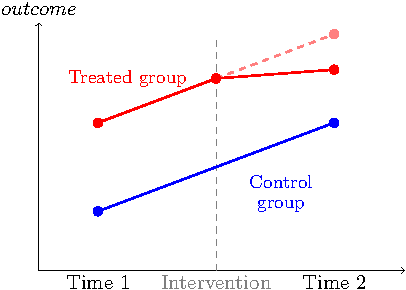
\includegraphics[width=0.5\textwidth,height=\textheight]{hei-report_files/figure-pdf/fig-didfig-1.pdf}

}

\caption{\label{fig-didfig}Stylized example of
difference-in-differences}

\end{figure}

The DiD design compares outcomes before and after an intervention in a
treated group relative to the same outcomes measured in a control group.
The control group trend provides the crucial ``counterfactual'' estimate
of what would have happened in the treated group had it not been
treated. By comparing each group to itself, this approach helps to
control for both measured and unmeasured fixed differences between the
treated and control groups. By measuring changes over time in outcomes
in the control group unaffected by the treatment, this approach also
controls for any unmeasured factors affecting outcome trends in both
treated and control groups. This is important since there are often many
potential factors affecting outcome trends that cannot be disentangled
from the policy if one only studies the treated group (as in a
traditional pre-post design).

The canonical DiD design (Card and Krueger 1994) compares two groups
(treated and control) at two different time periods (pre- and
post-intervention, Figure~\ref{fig-didfig}). In the first time period
both groups are untreated, and in the second time period one group is
exposed to the intervention. If we assume that the differences between
the groups would have remained constant in the absence of the
intervention (parallel trends assumption), then an unbiased estimate of
the impact of the intervention in the post period can be calculated by
subtracting the pre-post difference in the untreated group from the
pre-post difference in the treated group.

However, when multiple groups are treated at different time periods, the
most common approach has been to use a two-way fixed effects model to
estimate the impact of the intervention which controls for secular
trends and differences between districts. However, recent evidence
suggests that the traditional two-way fixed effects estimation of the
treatment effect may be biased in the context of heterogeneous treatment
effects (Callaway and Sant'Anna 2021; Goodman-Bacon 2021)

\hypertarget{measuring-pathways-and-mechanisms}{%
\subsection{Measuring pathways and
mechanisms}\label{measuring-pathways-and-mechanisms}}

To estimate how much of the CBHP intervention may work through different
mechanisms, we used causal mediation analysis. Causal approaches to
mediation attempt to discern between, and clarify the necessary
assumptions for identifying, different kinds of mediated effects. Taking
as an example the DAG in Figure~\ref{fig-dag1}, with \(T\) as the
policy, \(M\) as PM\textsubscript{2.5}, and \(Y\) as systolic blood
pressure, we can define the controlled direct effect (\(CDE\)) as the
effect of the CBHP policy on systolic blood pressure if we fix the value
of PM\textsubscript{2.5} to a certain reference level for the entire
population. For example, we can estimate the impact of the policy on
health outcomes while holding PM\textsubscript{2.5} at a uniform level
of average background exposure, or some other hypothetical level.

\begin{figure}[H]

{\centering 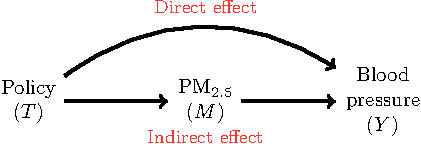
\includegraphics[width=0.5\textwidth,height=\textheight]{hei-report_files/figure-pdf/fig-dag1-1.pdf}

}

\caption{\label{fig-dag1}Example of direct and indirect effects with
outcome (\(Y\)), treatment (\(T\)), and mediator (\(M\))}

\end{figure}

Although other mediated effects such as ``natural'' direct and indirect
effects are theoretically estimable (VanderWeele 2015), they involve
challenging ``cross-world'' assumptions that are difficult to anchor in
policy (Naimi et al. 2014). Other approaches to mechanisms have focused
on principal stratification (e.g., Zigler et al. 2016), although
conceptual difficulties with identifying the (unverifiable) principal
strata make it challenging for questions of mediation. Because
controlled direct effects are considered more directly policy relevant
for public health, we focus on estimating these mediated quantities.

\hypertarget{data-analysis}{%
\section{Data Analysis}\label{data-analysis}}

To understand how the policy's impact on health may be mediated by
different potential mediators, we need to estimate first the total
effect of the policy on the outcomes, as well as the \(CDE\)s with
adjustment for potential mediators. As discussed above, in order for the
mediators to `explain' the total effects of the policy on health, the
policy should affect the mediators, and the mediators should also affect
the outcomes.

\hypertarget{total-effect}{%
\subsection{Total Effect}\label{total-effect}}

To estimate the total effect of the policy we used a DiD analysis that
accommodates staggered treatment rollout. To allow for heterogeneity in
the context of staggered rollout we used `extended' two-way fixed
effects (ETWFE) models (Wooldridge 2021) to estimate the total effect of
the CBHP policy. The mean outcome (replaced by a suitable link function
\(g(\cdot)\) for binary or count outcomes) was defined using a set of
linear predictors:

\begin{equation}\protect\hypertarget{eq-etwfe}{}{Y_{ijt}=g(\mu_{ijt}) = \alpha + \sum_{r=q}^{T} \beta_{r} d_{r} + \sum_{s=r}^{T} \gamma_{s} fs_{t}+ \sum_{r=q}^{T} \sum_{s=r}^{T} \tau_{rt} (d_{r} \times fs_{t}) + \varepsilon_{ijt}}\label{eq-etwfe}\end{equation}

where \(Y_{ijt}\) is the outcome for individual \(i\) in village \(j\)
at time \(t\), \(d_{r}\) represent treatment cohort dummies, i.e., fixed
effects for cohorts of villages that were first exposed to the policy at
the same time \(q\) (e.g., in 2019, 2020, or 2021), \(fs_{t}\) are time
fixed effects corresponding to different winter data collection
campaigns (2018-19, 2019-20, or 2021-22), and \(\tau_{rt}\) are the
cohort-time \emph{ATTs}. The ETWFE and other approaches that allow for
several (potentially heterogenous) treatment effects may also be
averaged to provide a weighted \(ATT\). Several potential possibilities
are feasible, including weighting by treatment cohorts or time since
policy adoption (Goin and Riddell 2023).

\hypertarget{mediation-analysis}{%
\subsection{Mediation Analysis}\label{mediation-analysis}}

As noted above, with respect to the mediation analysis we are chiefly
interested in the \(CDE\), which can be derived by adding relevant
mediators \(M\) to this model. If we also allow for exposure-mediator
interaction and potentially allow for adjustment for confounders \(W\)
of the mediator-outcome effect, we can extend equation
Equation~\ref{eq-etwfe} as follows:

\begin{equation}\protect\hypertarget{eq-etwfem}{}{
\begin{aligned}
Y_{ijt}=g(\mu_{ijt}) = \alpha + \sum_{r=q}^{T} \beta_{r} d_{r} + \sum_{s=r}^{T} \gamma_{s} fs_{t}+ \sum_{r=q}^{T} \sum_{s=r}^{T} \tau_{rt} (d_{r} \times fs_{t}) \\ + \delta M_{it} + \sum_{r=q}^{T} \sum_{s=r}^{T} \eta_{rt} (d_{r} \times fs_{t} \times M_{it}) + \zeta \mathbf{W} + \varepsilon_{ijt}
\end{aligned}
}\label{eq-etwfem}\end{equation}

where now \(\delta\) is the conditional effect of the mediator \(M\) at
the reference level of the treatment (again, represented via the series
of group-time interaction terms), and the collection of \(\eta\) terms
are coefficients for the product terms allowing for mediator-treatment
interaction. Finally, \(\zeta\) is a vector of coefficients for the set
of confounders contained within \(\mathbf{W}\).

As noted above, in the staggered DiD framework that allows for
heterogeneity, we do not have a single treatment effect but a collection
of group-time treatment effects that may be averaged in different ways.
This extends to the estimation of the \(CDE\), in which case we will
also have several \(CDE\)s that can be averaged to make inferences about
the extent to which the policy's impact is mediated by
\emph{PM\textsubscript{2.5}}. Based on the setup in
Equation~\ref{eq-etwfem} the \(CDE\) is estimated as:
\(\delta + \eta_{rt}MT\). In the absence of interaction between the
exposure and the mediator (i.e., \(\eta_{rt}=0\)) the \(CDE\) will
simply be the estimated treatment effects
\(\sum_{r=q}^{T} \sum_{s=r}^{T} \tau_{rt}\), i.e., the effect of the
policy holding \(M\) constant. For a valid estimate of the \(CDE\) we
must account for confounding of the mediator-outcome effect, represented
by \(W\) in the equation above. Baseline measures of both the outcome
and the proposed mediators inherent in our DiD strategy will help to
reduce the potential for unmeasured confounding of the mediator-outcome
effect (Keele et al. 2015).

\hypertarget{selection-of-confounders-and-effect-measure-modifiers}{%
\subsection{Selection of confounders and effect measure
modifiers}\label{selection-of-confounders-and-effect-measure-modifiers}}

\hypertarget{results-1}{%
\section{Results}\label{results-1}}

We retained all 50 villages in this four-year longitudinal assessment of
the CBHP in Beijing. By S2, S3, and S4 there were 10, 17, and 20 of the
50 study villages treated by the policy, respectively.
Figure~\ref{fig-flowchart} shows the participation across waves of data
collection. Throughout the entire study period, we enrolled a total of
\#\#\# participants in \#\#\# households and conducted a total of \#\#\#
individual-level observations. In each of the three campaigns with
individual and household-level measurements, we conducted measurements
in over 1000 study participants. Among the 1003 participants enrolled at
baseline, we obtained at least one follow-up measurement in 835
participants and two follow-up measurements in 667 participants. Among
the additional 276 participants recruited into the study in S2, we
obtained a second measurement in \#\# of these participants. There were
\#\# participants recruited into the study in S4 with just a single
measurement{[}g{]}.

Study flowchart

\begin{figure}[H]

{\centering 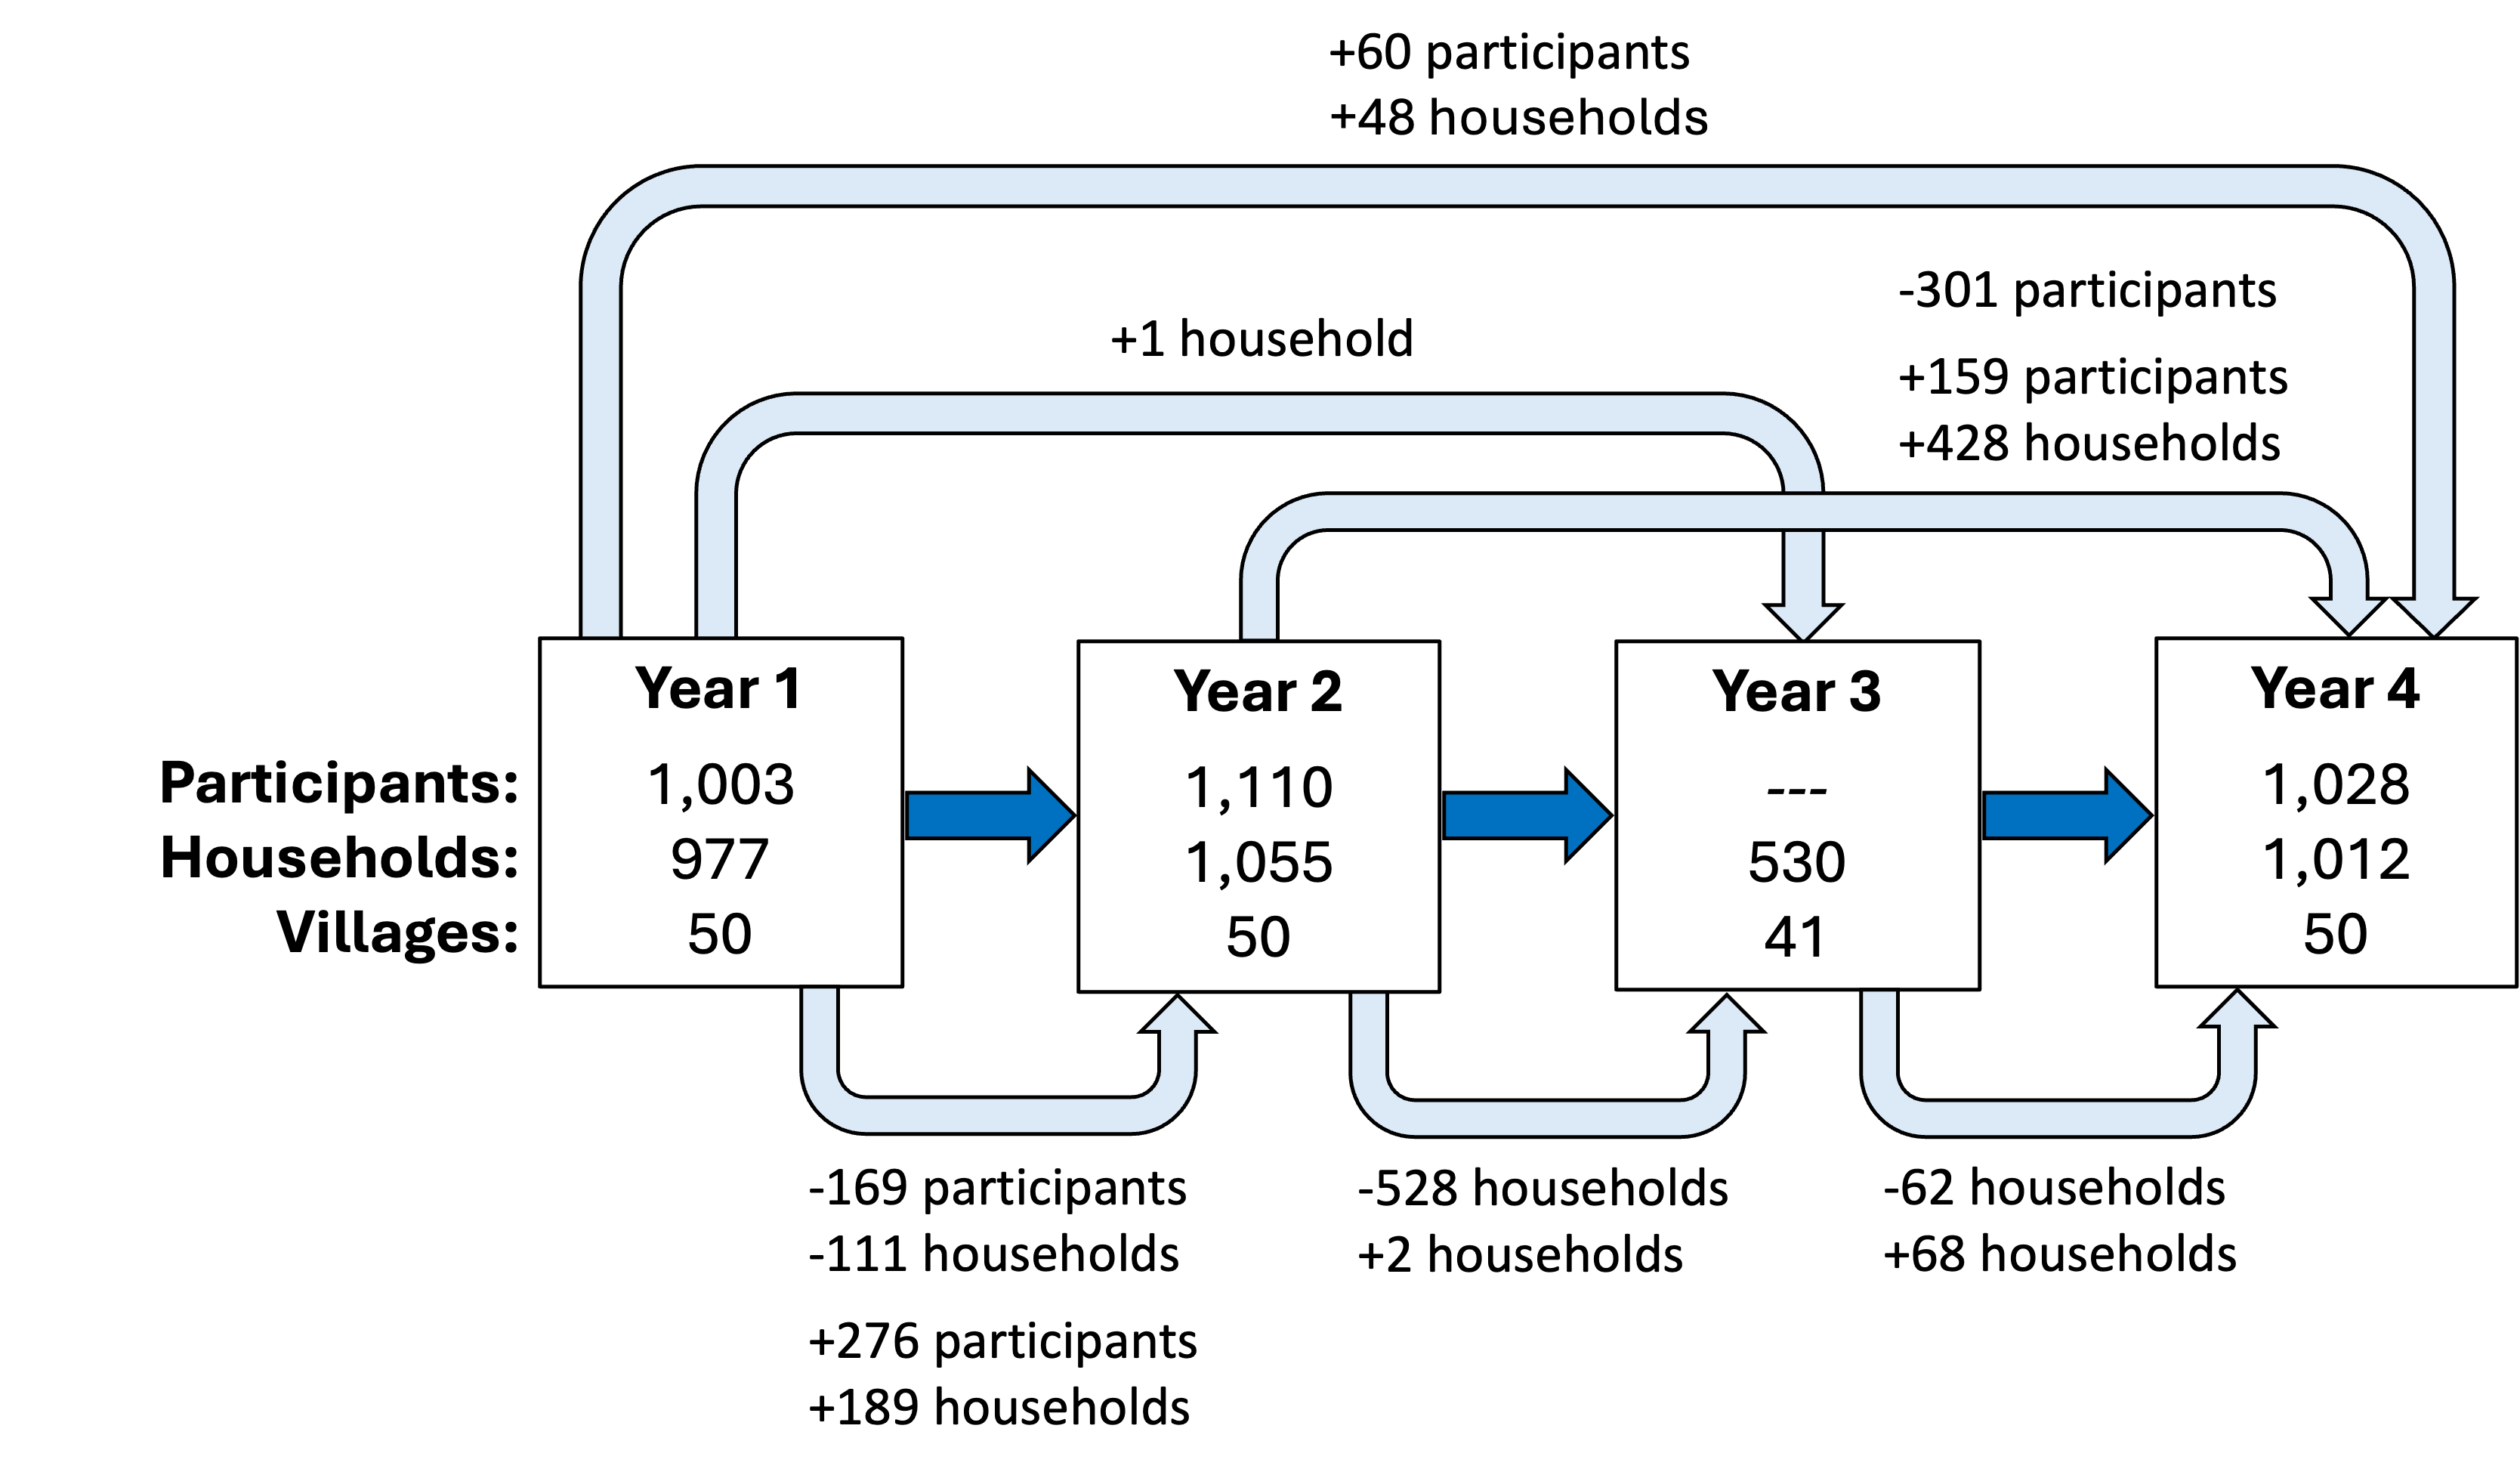
\includegraphics[width=0.8\textwidth,height=\textheight]{images/participation-flow-chart-Mar18.png}

}

\caption{\label{fig-flowchart}Flow chart of BHET study participation at
the participant, household, and village levels across study years.
Participation (number of units) in each study year is shown in the white
boxes. Additions (+) and losses (-) to the study sample between years
are indicated by the light blue arrows. Data collection was limited to
household- and village-level environmental measurements due to the
COVID-19 pandemic in year 3. We visited 530 households in 41 villages
before travel restrictions limited further data collection. This affects
the additions and losses to the study sample reported from years 2 to 3
and years 3 to 4.}

\end{figure}

\hypertarget{description-of-study-sample}{%
\subsection{Description of study
sample}\label{description-of-study-sample}}

\hypertarget{tbl-table1}{}
\begin{table}
\caption{\label{tbl-table1}Descriptive statistics for selected demographic, health, and
environmental measures at baseline, by treatment status }\tabularnewline

\centering\centering
\fontsize{9}{11}\selectfont
\begin{tabular}[t]{rrrrrrr}
\toprule
\multicolumn{1}{c}{ } & \multicolumn{2}{c}{Never treated (N=603)} & \multicolumn{2}{c}{Ever treated (N=400)} & \multicolumn{2}{c}{ } \\
\cmidrule(l{3pt}r{3pt}){2-3} \cmidrule(l{3pt}r{3pt}){4-5}
  & Mean & Std. Dev. & Mean & Std. Dev. & Diff. in Means & Std. Error\\
\midrule
\textbf{Demographics:} & \textbf{} & \textbf{} & \textbf{} & \textbf{} & \textbf{} & \textbf{}\\
Age (years) & 59.9 & 9.4 & 60.4 & 9.2 & 0.5 & 0.6\\
Female (\%) & 59.5 & 49.1 & 59.1 & 49.2 & -0.4 & 3.2\\
No education (\%) & 11.5 & 31.9 & 12.3 & 32.9 & 0.9 & 2.1\\
Primary education (\%) & 75.5 & 43.0 & 77.6 & 41.7 & 2.1 & 2.8\\
Secondary+ education (\%) & 12.6 & 33.2 & 9.8 & 29.7 & -2.9 & 2.0\\
\textbf{Health measures:} & \textbf{} & \textbf{} & \textbf{} & \textbf{} & \textbf{} & \textbf{}\\
Never smoker (\%) & 61.9 & 48.6 & 59.5 & 49.1 & -2.4 & 3.2\\
Former smoker (\%) & 11.9 & 32.4 & 15.1 & 35.8 & 3.2 & 2.2\\
Current smoker (\%) & 26.2 & 44.0 & 25.4 & 43.6 & -0.8 & 2.8\\
Never drinker (\%) & 55.9 & 49.7 & 52.5 & 50.0 & -3.4 & 3.2\\
Occasional drinker (\%) & 26.0 & 43.9 & 25.5 & 43.6 & -0.5 & 2.8\\
Daily drinker (\%) & 17.8 & 38.3 & 21.9 & 41.4 & 4.1 & 2.6\\
Systolic (mmHg) & 131.4 & 16.8 & 128.7 & 14.3 & -2.7 & 1.0\\
Diastolic (mmHg) & 82.7 & 11.6 & 82.1 & 11.3 & -0.6 & 0.8\\
Waist circumference (cm) & 87.7 & 10.5 & 85.4 & 9.5 & -2.3 & 0.8\\
Body mass index (kg/m2) & 26.3 & 3.7 & 25.8 & 3.6 & -0.5 & 0.3\\
Frequency of coughing (\%) & 18.7 & 39.0 & 19.7 & 39.8 & 1.0 & 2.6\\
Frequency of wheezing (\%) & 6.2 & 24.2 & 6.6 & 24.8 & 0.3 & 1.6\\
Shortness of breath (\%) & 29.2 & 45.5 & 34.3 & 47.5 & 5.1 & 3.0\\
Chest trouble (\%) & 11.6 & 32.0 & 14.1 & 34.9 & 2.5 & 2.2\\
Any respiratory problem (\%) & 50.6 & 50.0 & 54.3 & 49.9 & 3.7 & 3.2\\
\textbf{Environmental measures:} & \textbf{} & \textbf{} & \textbf{} & \textbf{} & \textbf{} & \textbf{}\\
Temperature (°C) & 13.8 & 3.6 & 13.5 & 3.3 & -0.3 & 0.2\\
Personal PM2.5 (ug/m3) & 150.2 & 300.3 & 103.8 & 107.3 & -46.3 & 19.1\\
\bottomrule
\multicolumn{7}{l}{\rule{0pt}{1em}Includes all individuals sampled at each of 3 waves.}\\
\end{tabular}
\end{table}

Table~\ref{tbl-table1} shows the distribution of selected demographic,
health, and environmental characteristics from the baseline survey,
prior to any villages being enrolled in the ban. We provide means and
standard deviations separately for villages that eventually enter into
the ban with those that never do so. As noted above, although our DiD
identification strategy allows for fixed differences between treated and
untreated villages, overall the differences at baseline are generally
small and the groups seem well balanced on most measures, with the
exception of personal PM\textsubscript{2.5} exposure, which was lower in
villages that were eventually treated.

\hypertarget{summary-of-pm-and-bc-measurements}{%
\subsection{Summary of PM and BC
measurements}\label{summary-of-pm-and-bc-measurements}}

At baseline, fine particulate matter (PM\textsubscript{2.5}) and black
carbon (BC) concentrations were highest, on average, for personal
exposures compared with indoor and outdoor concentrations, with indoor
levels being higher than outdoors (Figure~\ref{fig-pm-baseline}). This
trend (personal \textgreater{} indoor \textgreater{} outdoor) was
observed among households in treated and untreated villages. Personal,
indoor, and outdoor geometric mean (95\% confidence interval)
concentrations of PM\textsubscript{2.5} were 72 (65,80), 45 (39,53), and
31 (28,35), respectively, and elevated relative to health-based
guidelines. The current World Health Organization (WHO) guidelines state
that annual average concentrations of PM\textsubscript{2.5} should not
exceed 5 µg/m3, while 24-hour average exposures should not exceed 15
µg/m3 more than 3 - 4 days per year (Organization 2021). Interim targets
have been set to support the planning of incremental milestones toward
cleaner air, particularly for cities, regions, and countries with higher
air pollution levels. For PM\textsubscript{2.5}, the four interim (IT)
targets for annual and 24-h means are: IT-1: 35 and 75 µg/m3; IT-2: 25
and 50 µg/m3; IT-3: 15 and 37.5 µg/m3; and IT-4: 10 and 25 µg/m3
(Organization 2021). In our study, baseline air pollution exposures and
indoor concentrations were between IT-3 and IT-4, indicating
considerable opportunity for air quality improvement.

\begin{figure}[H]

{\centering 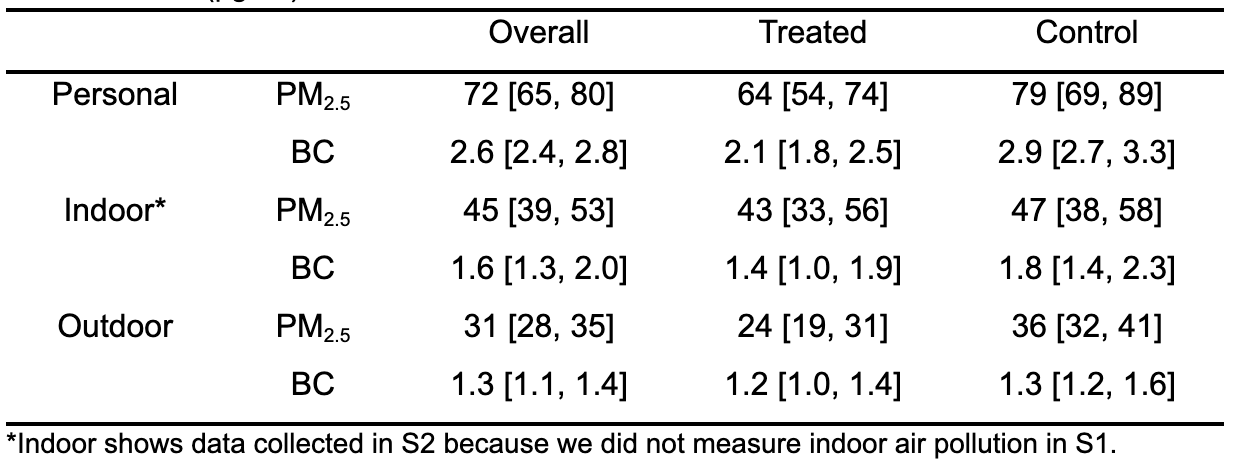
\includegraphics[width=0.8\textwidth,height=\textheight]{images/fig-pm-baseline.png}

}

\caption{\label{fig-pm-baseline}Geometric mean and 95\% Confidence
Intervals for filter-based air pollutant concentrations at baseline.}

\end{figure}

\hypertarget{policy-uptake}{%
\subsection{Policy uptake}\label{policy-uptake}}

Each year of the study, participants reported the types of fuels and
stoves used for space heating in winter. Based on these data, heating
energy types were classified into four categories: exclusive use of a
heat pump (`heat pump exclusively'), use of a heat pump and a kang
(`heat pump with kang'), use of solid fuel with use of electric heating
devices other than heat pumps (`solid fuel with electricity (not heat
pump)'), and exclusive use of solid fuel. In villages treated under the
policy, Figure~\ref{fig-sankey} shows meaningful transitions from solid
fuel to heat pumps for all treatment cohorts. For example, in villages
treated in S2, over 90\% of households used heat pumps in S2, increasing
to 96\% in S4, while only 3\% used heat pumps in S1. Conversely, the use
of coal stoves decreased from 97\% in S1 to 8\% in S2 and 3\% in S4.
Villages treated in S4 initially relied heavily on solid fuel, with
approximately 90\% of households reporting use of solid fuels in S1 and
S2. However, after treatment, 94\% of households in these same villages
reported using heat pumps in S4.

We also observed a substantial decline in self-reported coal use when
villages entered into the CBHP policy (Appendix
Figure~\ref{fig-afig-coal}). Reductions in coal use were consistent
across coal types, including both honeycomb briquettes (reported by
number of briquettes) and traditional coal (reported by the ton). At the
same time, participant-reported wintertime expenditures (reported in
Chinese Yuan) on electricity in each year of the study increased once
villages entered the CBHP policy. Biomass (i.e., wood logs/twigs or
charcoal) represents another source of heating fuel not expressly
targeted by the CBHP policy. In villages treated in S2 and S3, the use
of wood declined once villages entered the policy, but not to the same
degree as coal use declined. In villages treated in S4 -- albeit a small
number (n=3 villages) -- the use of wood showed a slight increase after
treatment.

In untreated villages, an active transition from solid fuel to clean
energy was also observed during our four year study period. The use of
heat pumps increased gradually from 5\% in S1 to 10\% in S2 and 25\% in
S4. Commensurately, the reported expenditures on electricity increased
gradually over time in the untreated villages (Appendix
Figure~\ref{fig-afig-coal}). The percentage of untreated households
using solid fuel with electric devices remained relatively stable,
ranging from 64\% to 70\%. The use of wood fuel remained stable, as
well, at approximately one ton of fuel per winter. However, exclusive
use of solid fuel decreased from 30\% in S1 to 7\% in S4.

\begin{figure}[H]

{\centering 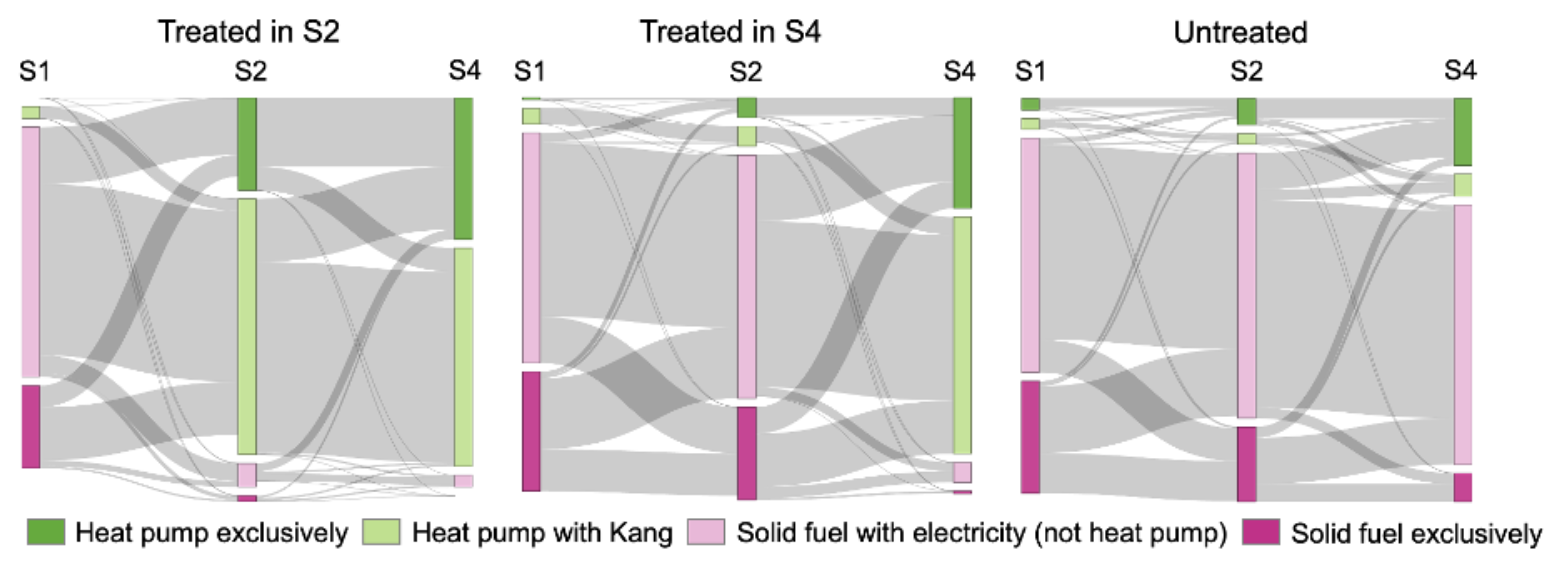
\includegraphics[width=1\textwidth,height=\textheight]{images/sankey.png}

}

\caption{\label{fig-sankey}Transitions to different energy sources
across study seasons}

\end{figure}

\hypertarget{aim-1-policy-impacts-and-potential-mediation}{%
\subsection{Aim 1: Policy impacts and potential
mediation}\label{aim-1-policy-impacts-and-potential-mediation}}

\hypertarget{impact-of-policy-on-potential-mediators}{%
\subsubsection{Impact of policy on potential
mediators}\label{impact-of-policy-on-potential-mediators}}

In estimating the treatment effect on indoor and outdoor air pollution,
we evaluated both 24-h mean values (specifically, the same 24-h period
when personal exposure samples were collected in each village) and
seasonal mean values (with `season' defined from Jan.~15th to Mar.~15th)
of PM2.5 data collected in each village. For estimating the treatment
effect on personal exposure to PM2.5 and black carbon (BC), the results
from the filter-based measurements that were collected for a 24-h period
were used for analysis. We estimated the basic ETWFE models, as well as
ETWFE models further adjusted for covariates, including temperature,
relative humidity, wind speed, boundary layer height, wind direction,
and the mean quantity of wood burned in each village).

\hypertarget{tbl-did-med}{}
\begin{table}
\caption{\label{tbl-did-med}Treatment effect on outdoor and indoor PM2.5, as well as personal
exposure to PM2.5 and black carbon. Outdoor and indoor PM2.5 were
derived from sensor measurements after being adjusted based on
co-located gravimetric PM2.5 measurements. `Daily' indicates the mean
PM2.5 concentrations during the 24 hours when personal exposure samples
were collected in each village. `Seasonal' indicates the seasonal mean
PM2.5 concentrations in each village, from Jan. 15th to Mar. 15th. `Did'
represents the DiD analysis without any covariates, while `Adjusted DiD'
represents DiD analysis with covariates. }\tabularnewline

\centering
\begin{tabular}{llcccc}
\toprule
\multicolumn{2}{c}{ } & \multicolumn{2}{c}{DiD} & \multicolumn{2}{c}{Adjusted DiD*} \\
\cmidrule(l{3pt}r{3pt}){3-4} \cmidrule(l{3pt}r{3pt}){5-6}
  &   & Estimate & (95\% CI) & Estimate & (95\% CI)\\
\midrule
\addlinespace[0.3em]
\multicolumn{6}{l}{\textbf{Air pollution (µg/m3)}}\\
\hspace{1em} & PM2.5 & -2.09 & (-29.38, 25.2) & 1.95 & (-23.34, 27.23)\\
\cmidrule{2-6}
\multirow[t]{-2}{*}[1\dimexpr\aboverulesep+\belowrulesep+\cmidrulewidth]{\raggedright\arraybackslash Personal} & Black carbon & -0.46 & (-1.73, 0.81) & -0.43 & (-1.67, 0.81)\\
\cmidrule{1-6}
\hspace{1em} & Daily & -19.10 & (-60.56, 22.35) & -15.38 & (-53.54, 22.78)\\
\cmidrule{2-6}
\multirow[t]{-2}{*}[1\dimexpr\aboverulesep+\belowrulesep+\cmidrulewidth]{\raggedright\arraybackslash Indoor} & Seasonal & -35.11 & (-59.36, -10.85) & -36.27 & (-60.26, -12.29)\\
\cmidrule{1-6}
\hspace{1em} & Daily & -0.11 & (-5.86, 5.64) & -1.73 & (-9.26, 5.81)\\
\cmidrule{2-6}
\multirow[t]{-2}{*}[1\dimexpr\aboverulesep+\belowrulesep+\cmidrulewidth]{\raggedright\arraybackslash Outdoor} & Seasonal & 3.14 & (-3.1, 9.38) & 0.36 & (-6.27, 6.99)\\
\cmidrule{1-6}
\addlinespace[0.3em]
\multicolumn{6}{l}{\textbf{Indoor temperature (°C)}}\\
\hspace{1em}Point temp & Mean & 1.96 & (0.96, 2.96) & \textbackslash{} & \\
\bottomrule
\multicolumn{6}{l}{\rule{0pt}{1em}\textsuperscript{*} Footnote A}\\
\end{tabular}
\end{table}

Treatment was associated with similar reductions in both seasonal and
24-h indoor PM\textsubscript{2.5} means (Table~\ref{tbl-did-med}). On
average, treatment was associated with a decrease in 24-h indoor
PM\textsubscript{2.5} of -38 {[}-75, -1{]} μg/m3. After adjusting for
covariates such as outdoor temperature, dewpoint, household smoking
status, and the number of residents in each household, the treatment
effect decreased to -31 {[}-64, -2{]} μg/m3. The treatment effect on
seasonal indoor PM2.5 (-39 {[}-55, -23{]} μg/m3) remained consistent
after covariate adjustment. This finding likely reflects the direct
benefit of the policy in replacing coal stoves, thereby improving indoor
air quality.

Overall we found little evidence of an impact of the CBHP policy on 24-h
and seasonal outdoor (local community-level) PM\textsubscript{2.5} or
personal exposures to PM\textsubscript{2.5} and BC. Treatment was
associated with lower, but statistically imprecise, personal 24-h BC
exposures. This finding would be consistent with the expectation that
the policy contributed to reducing air pollutant emissions from solid
fuel burning, as BC serves as a potential indicator of such combustion,
particularly in our study settings.

\hypertarget{impact-of-policy-on-health-outcomes}{%
\subsubsection{Impact of policy on health
outcomes}\label{impact-of-policy-on-health-outcomes}}

\hypertarget{tbl-did-health}{}
\begin{table}
\caption{\label{tbl-did-health}Overall impacts of the `coal-to-clean energy' policy on blood pressure,
respiratory outcomes, and inflammatory markers }\tabularnewline

\centering
\begin{tabular}{llcccc}
\toprule
\multicolumn{2}{c}{ } & \multicolumn{2}{c}{DiD} & \multicolumn{2}{c}{Adjusted DiD*} \\
\cmidrule(l{3pt}r{3pt}){3-4} \cmidrule(l{3pt}r{3pt}){5-6}
  &   & Estimate & (95\% CI) & Estimate & (95\% CI)\\
\midrule
\addlinespace[0.3em]
\multicolumn{6}{l}{\textbf{Blood pressure (mmHg)}}\\
\hspace{1em} & Brachial & -0.79 & (-2.63, 1.04) & -1.40 & (-3.31, 0.51)\\
\cmidrule{2-6}
\multirow[t]{-2}{*}[1\dimexpr\aboverulesep+\belowrulesep+\cmidrulewidth]{\raggedright\arraybackslash Systolic BP} & Central & -1.04 & (-2.82, 0.73) & -1.56 & (-3.40, 0.28)\\
\cmidrule{1-6}
\hspace{1em} & Brachial & -1.29 & (-2.62, 0.04) & -1.60 & (-2.96, -0.25)\\
\cmidrule{2-6}
\multirow[t]{-2}{*}[1\dimexpr\aboverulesep+\belowrulesep+\cmidrulewidth]{\raggedright\arraybackslash Diastolic BP} & Central & -1.35 & (-2.66, 0.04) & -1.66 & (-2.97, -0.34)\\
\cmidrule{1-6}
\hspace{1em} & Brachial & 0.50 & (-0.71, 1.70) & 0.21 & (-1.00, 1.41)\\
\cmidrule{2-6}
\multirow[t]{-2}{*}[1\dimexpr\aboverulesep+\belowrulesep+\cmidrulewidth]{\raggedright\arraybackslash Pulse Pressure} & Central & 0.31 & (-0.85, 1.46) & 0.10 & (-1.01, 1.20)\\
\cmidrule{1-6}
\hspace{1em} & Pulse pressure & 0.10 & (-0.12, 1.40) & 0.00 & (-1.20, 1.20)\\
\cmidrule{2-6}
\multirow[t]{-2}{*}[1\dimexpr\aboverulesep+\belowrulesep+\cmidrulewidth]{\raggedright\arraybackslash BP Amplification x10} & Systolic BP & 0.20 & (-0.20, 0.50) & 0.10 & (-0.20, 0.40)\\
\cmidrule{1-6}
\addlinespace[0.3em]
\multicolumn{6}{l}{\textbf{\makecell[l]{Respiratory\\outcomes}}}\\
\hspace{1em} & Any symptom & -7.38 & (-13.98, -0.77) & -7.86 & (-14.63, -1.09)\\
\cmidrule{2-6}
\hspace{1em} & Coughing & -1.59 & (-6.41, 3.23) & -1.98 & (-6.8, 2.84)\\
\cmidrule{2-6}
\hspace{1em} & Phlegm & -1.22 & (-5.58, 3.15) & -1.82 & (-6.34, 2.69)\\
\cmidrule{2-6}
\hspace{1em} & Wheezing attacks & -0.22 & (-3.97, 3.52) & -0.14 & (-3.85, 3.57)\\
\cmidrule{2-6}
\hspace{1em} & Trouble breathing & -4.98 & (-11.81, 1.84) & -4.62 & (-11.59, 2.35)\\
\cmidrule{2-6}
\multirow[t]{-6}{*}[5\dimexpr\aboverulesep+\belowrulesep+\cmidrulewidth]{\raggedright\arraybackslash Self-reported (pp)} & Chest trouble & -6.63 & (-12.51, -0.76) & -6.36 & (-12.14, -0.59)\\
\cmidrule{1-6}
\hspace{1em}Measured & FeNO (ppb) & 0.17 & (-2.24, 2.58) & 0.55 & (-2.13, 3.13)\\
\cmidrule{1-6}
\addlinespace[0.3em]
\multicolumn{6}{l}{\textbf{\makecell[l]{Inflammatory\\markers (\%)}}}\\
\hspace{1em} & IL6 & 6.80 & (-12.2, 30.0) & 5.90 & (-13.8, 30.2)\\
\cmidrule{2-6}
\hspace{1em} & TNF-alpha & 24.30 & (-1.3, 56.4) & 24.70 & (-0.9, 54.2)\\
\cmidrule{2-6}
\hspace{1em} & CRP & 2.70 & (-19.8, 31.6) & 3.80 & (-19.4, 33.6)\\
\cmidrule{2-6}
\multirow[t]{-4}{*}[3\dimexpr\aboverulesep+\belowrulesep+\cmidrulewidth]{\raggedright\arraybackslash } & MDA & 7.60 & (-8.7, 26.9) & 6.50 & (-9.7, 25.5)\\
\bottomrule
\multicolumn{6}{l}{\rule{0pt}{1em}\textit{Note: } pp = percentage points, ppb = parts per billion}\\
\multicolumn{6}{l}{\rule{0pt}{1em}\textsuperscript{*} List of adjustments...}\\
\end{tabular}
\end{table}

Table~\ref{tbl-did-health} shows the impacts of the policy on blood
pressure in basic ETWFE models and models further adjusted for age, sex,
waist circumference, smoking, alcohol consumption, and use of blood
pressure medication. Overall exposure to the CBHP policy demonstrated
reductions in blood pressure of approximately 1.5 mmHg systolic and
diastolic BP, but we found little evidence of a meaningful impact on
pulse pressure or BP amplification. The effects on brachial and central
blood pressures were similar.

Table~\ref{tbl-did-health} shows the impacts on self-reported chronic
respiratory symptoms categorized as any symptoms and separately for each
individual symptom type. In both basic and covariate-adjusted ETWFE
models, exposure to the CBHP policy reduced self-report of any poor
respiratory symptoms by around 7 percentage points. This was largely
through reductions in reports of having chest trouble or difficulty
breathing on several or most days of the week.

Table~\ref{tbl-did-health} shows the impacts of the CBHP on measured
airway inflammation (FeNO), which was conducted in a sub-sample of 511
participants, including 274 participants with one measurement, 142 with
two measurements, 95 participants with 3 measurements. We did not find
evidence that exposure to the policy affected changes in FeNO in the
covariate-adjusted ETWFE model (0.5 ppb, 95\%CI: -2.1, 3.1) (Table X).
There was some evidence of heterogeneity in the FeNO effects of the
policy by treatment cohort{[}h{]} but the confidence intervals for each
of the cohort-specific effects were large and overlapping. Our results
did not change with sensitivity analyses that included a log-transformed
FeNO outcome and limiting the analysis to participants with at least two
repeated measurements and to those who participated in all three
campaigns (SI Table X)

\hypertarget{mediated-impact-on-blood-pressure}{%
\subsection{Mediated impact on blood
pressure}\label{mediated-impact-on-blood-pressure}}

As noted above, we aimed to assess whether any health impacts of the
CBHP policy may work specifically through pathways involving changes in
PM\textsubscript{2.5} and indoor temperature. Below we show results from
several mediation models. We evaluated potential mediation for each
mediator separately and in a single model accounting for multiple
mediators, and we set the values of both mediators to the WHO mean
annual interim PM\textsubscript{2.5} and indoor temperature guidelines.
For mediation analysis, we focused on BP outcomes for which we observed
an effect of the policy. In Table~\ref{tbl-bp-med} we show that
conditioning on indoor PM and indoor temperature largely explains the
entire total effect of the CBHP policy on blood pressure for systolic
BP, and roughly half of the total effect for diastolic BP.

\hypertarget{tbl-bp-med}{}
\begin{table}[H]
\caption{\label{tbl-bp-med}Controlled direct effects for the CBHP policy }\tabularnewline

\centering
\begin{tabular}{lllll}
\toprule
\multicolumn{2}{c}{ } & \multicolumn{3}{c}{CDE Mediated By:} \\
\cmidrule(l{3pt}r{3pt}){3-5}
Outcome & Adjusted Total Effect & Indoor PM & Indoor Temp & PM + Temp\\
\midrule
Brachial SBP & -1.4 (-3.31, 0.51) & -0.93 (-3.05, 1.2) & -0.43 (-2.35, 1.49) & 0.13 (-2.02, 2.28)\\
Central SBP & -1.56 (-3.4, 0.28) & -1.02 (-3.13, 1.08) & -0.54 (-2.39, 1.3) & 0.07 (-2.05, 2.19)\\
Brachial DBP & -1.6 (-2.96, -0.25) & -1.3 (-2.81, 0.21) & -1.02 (-2.45, 0.42) & -0.65 (-2.25, 0.94)\\
Central DBP & -1.66 (-2.97, -0.34) & -1.31 (-2.81, 0.19) & -1.08 (-2.48, 0.32) & -0.68 (-2.27, 0.9)\\
\bottomrule
\end{tabular}
\end{table}

\hypertarget{aim-2-source-contributions}{%
\subsection{Aim 2: Source
contributions}\label{aim-2-source-contributions}}

We first performed descriptive analyses (range, mean, standard
deviation, median, and interquartile range) for community-outdoor,
indoor, and personal exposure to air pollution, by data collection
campaign, by village, and by households within villages. We evaluated
factors contributing to PM\textsubscript{2.5} (community-outdoor and
personal exposure) using the U.S. EPA's source apportionment model PMF
(positive matrix factorization) 5.0, which has been widely used for
similar analyses in China (Gao et al.~2018; Liu et al.~2017; Tao et
al.~2017). As an optimum PMF result depends on the appropriate number of
input factors, sensitivity analysis using a range of factors (range of 3
to 7 factors, based on a combination of the species that we have and our
field-based observations and sources that have been identified
previously in our study region) were conducted to examine the impact of
a different number of factors on the model results. Detailed information
on the procedures of PMF analysis can be found elsewhere (Wang et
al.~2016; Zíková et al.~2016). Based on the scree plot from our
principal component analysis indicated that solutions of between 3 and 5
factors (+/- 1) would be most appropriate, further supporting our
evaluation of 3 to 6 factor solutions from PMF. There was no indication
(Table X) that even moving from five factors to six factors would
improve our solution; therefore, a seven factor solution would not make
sense to investigate further.

For our analysis, we additionally applied recently developed methods
that account for the impact of meteorological conditions in the PMF
analysis. This new approach is referred to as dispersion-normalized (DN)
PMF. Essentially, this approach scales \ldots{[}i{]}

Source analysis for this study was conducted using data from all
eligible outdoor PM and personal PM samples. Eligible samples were
defined as \ldots{}

The model diagnostics for the three- to six-factor PMF solutions are
given in Figure~\ref{fig-source-table}. Model fit was assessed using
Q/Qexp (how our model fit divided by the expected fit). As the change in
Q/Qexp decreases as more factors are added, the model may be fitting
additional sources that do not improve the overall fit. The largest
change in Q/Qexp was from three to four sources (6.24 to 5.37) while the
changes moving from four to five and five to six are similar which
suggests that four factors is sufficient and parsimonious to explain the
variation in our data. We assessed the random error in our model by
randomly sampling blocks of data, fitting new models with the blocks,
and comparing how the source profiles compared to that of the original
model (BS mapping). The three- and four-factor solutions had high BS
mapping (all factors found in \textgreater{} 96.5\% of bootstrap runs).
The additional sources identified in the five-factor (lead) and
six-factor (chloride) solutions have low bootstrap mapping
(\textgreater{} 72\%), which means those solutions are not as consistent
as the three- and four-factor solutions. The possibility that multiple,
different, solutions could result in the same Q value was assessed using
displacement. The displacement approach takes the original factor
profiles and modifies the values for each species up or down to maintain
a small change in Q, reruns the solution with the new species values,
and then compares the profiles of the new model to the original. Any
swaps indicate that small changes in the species values could result in
factor profiles that look different from the original solution, and that
the original solution is unstable. None of the factors in any of the
solutions discussed were swapped during displacement, which indicates
that all of the potential solutions are stable. Based on the Q/Qexp, BS
mapping, and interpretability of the factors, the four-factor solution
was selected as the most appropriate source solution for the data.

\begin{figure}[H]

{\centering 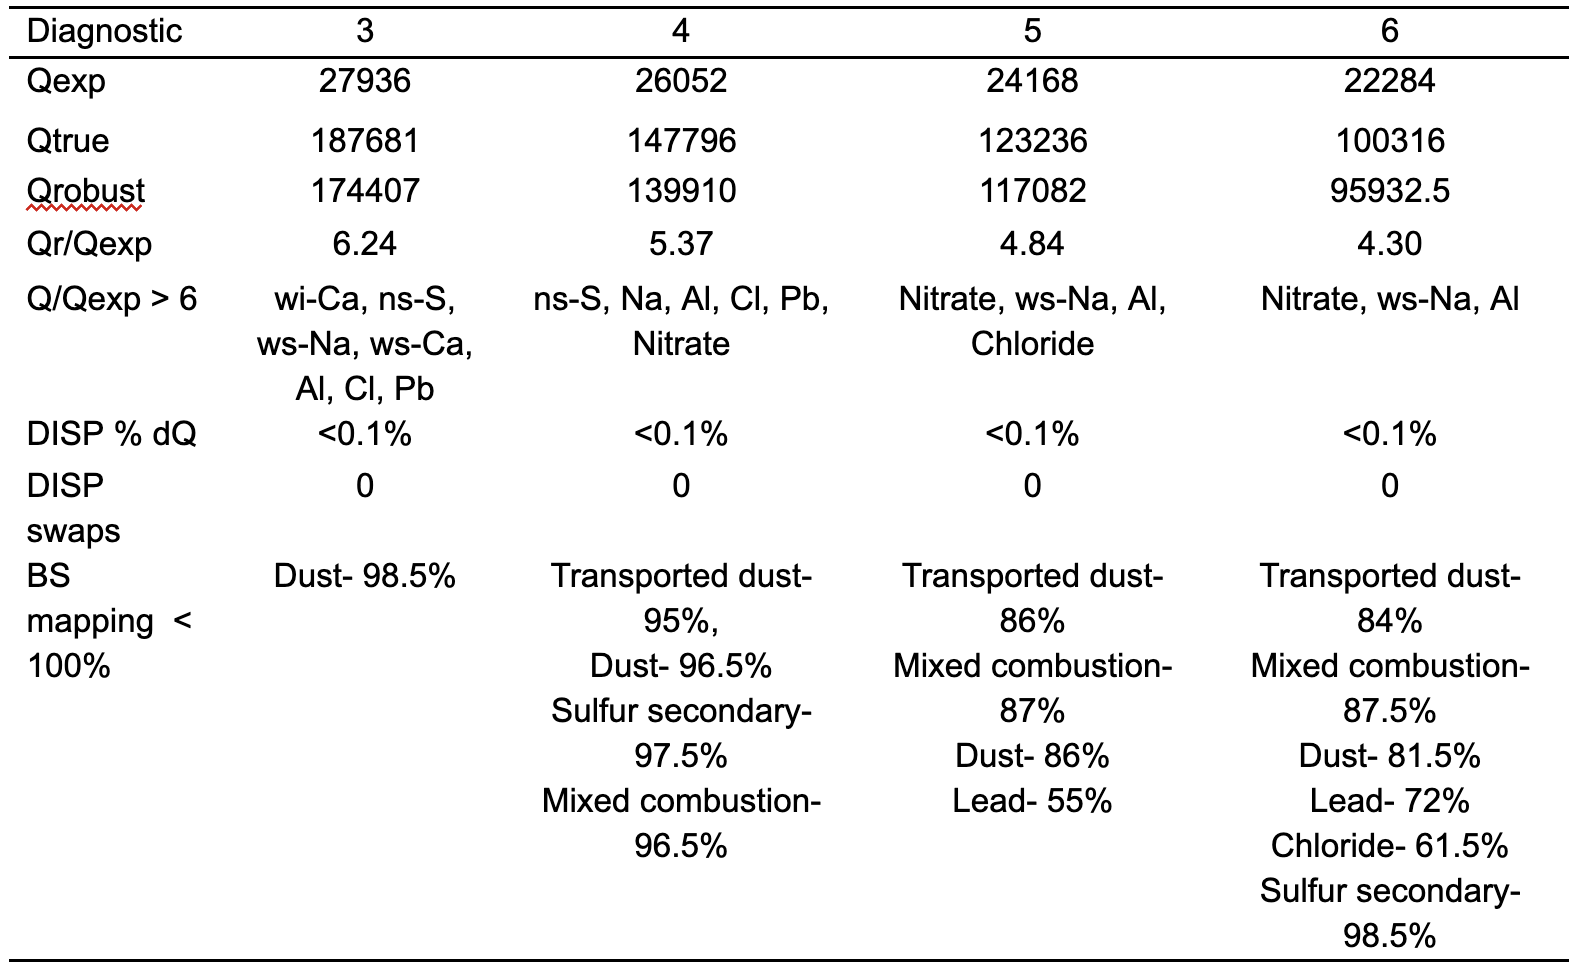
\includegraphics[width=0.8\textwidth,height=\textheight]{images/source-table.png}

}

\caption{\label{fig-source-table}PMF error estimation diagnostics.}

\end{figure}

The source profiles for the four-factor solution are presented in
Figure~\ref{fig-source-figure}. The first source was identified as dust
by high percentages of crustal elements like wi-Ca, Si, and wi-Mg. The
second source was constituted of non-sulfate sulfur as well as secondary
inorganic ions (ammonium, nitrate, and sulfate). Non-sulfate sulfur is a
tracer for primary coal combustion, while secondary inorganic ions
indicate a secondary source. Since coal combustion is a major source of
energy in our study area, it is likely that the second source is a
mixture of primary and secondary emissions that originate from coal and
other sulfurous fuel combustion. Additionally, the mean source
contribution of the second source is higher in outdoor than personal
exposure measurements. Secondary formation occurs outdoors in the
presence of sunlight, so higher outdoor concentrations compared to
personal exposure further support our naming the second source and
sulfur secondary. The third source had high percentages of ws-Ca nd Al,
which in our study region, has been found to be indicative of
transported dust from dust storms that can occur in the spring. While
our samples were collected during winter months only, it is possible
that transported dust from previous years still remained. The fourth
source was characterized by high percentages of tracers for both coal
(OC, wi-K, chloride, Pb) and biomass combustion (EC, ws-K). Coal and
biomass combustion is common in our study setting so this source is
likely a mixture of the two combustion sources.

\begin{figure}[H]

{\centering 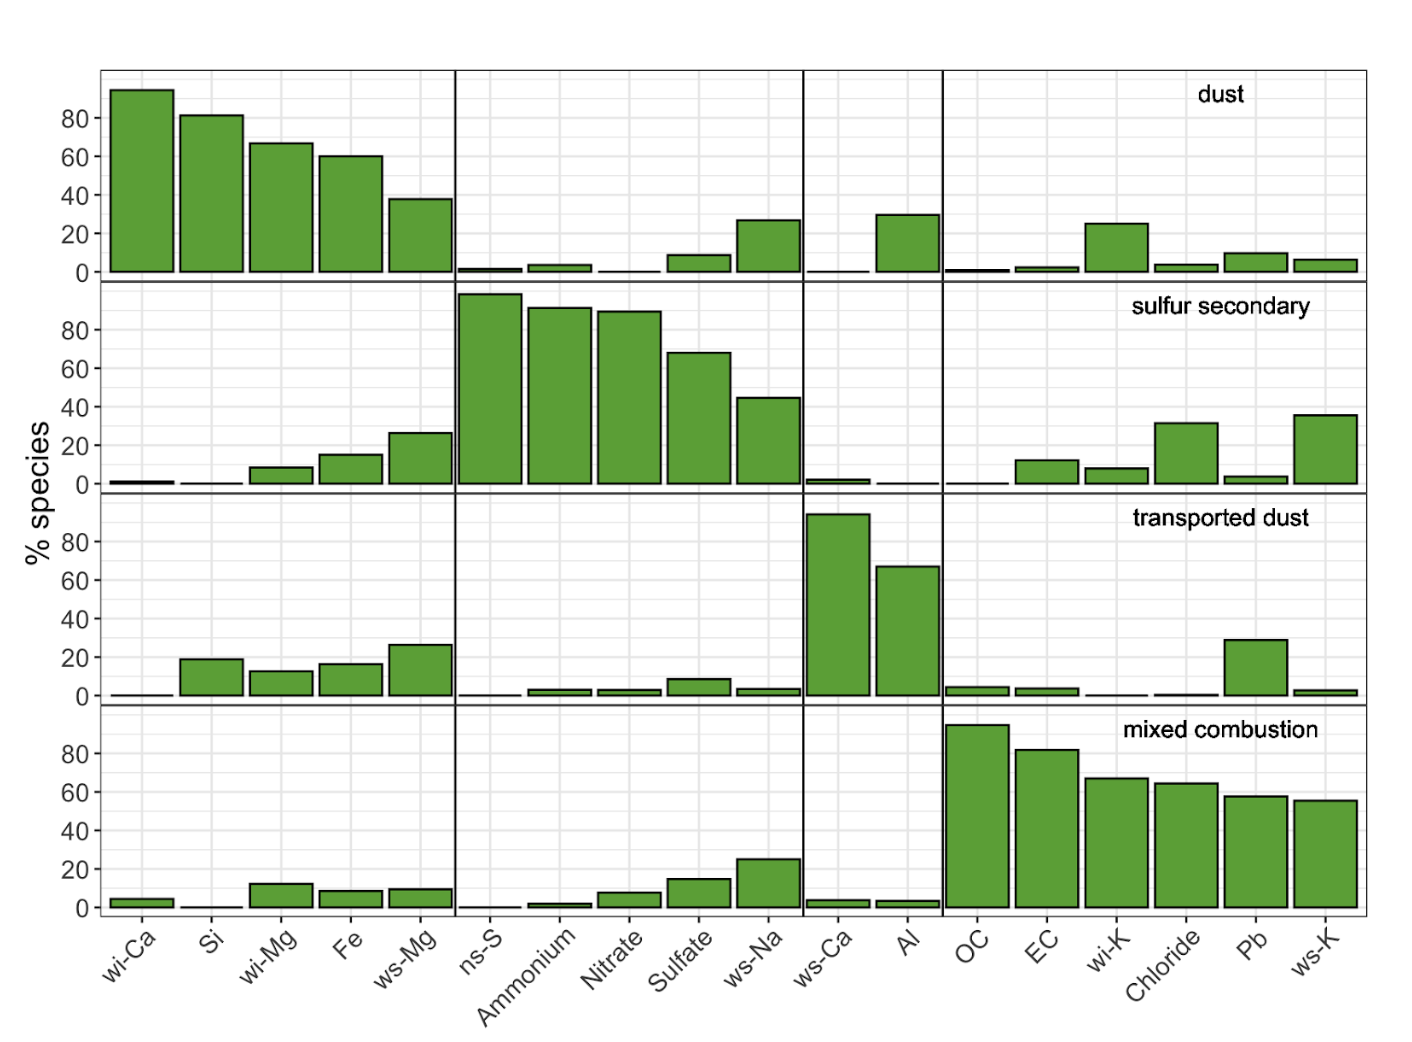
\includegraphics[width=0.8\textwidth,height=\textheight]{images/source-figure.png}

}

\caption{\label{fig-source-figure}Source profiles for the 4-factor PMF
solution to the sum of elements, ions, elemental carbon, and organic
carbon for outdoor and personal PM2.5 exposure measurements. The lines
separate the major contributing species to each source}

\end{figure}

We extend the source profiles across the different treatment cohorts in
Figure~\ref{fig-source-season}.

\begin{figure}[H]

{\centering 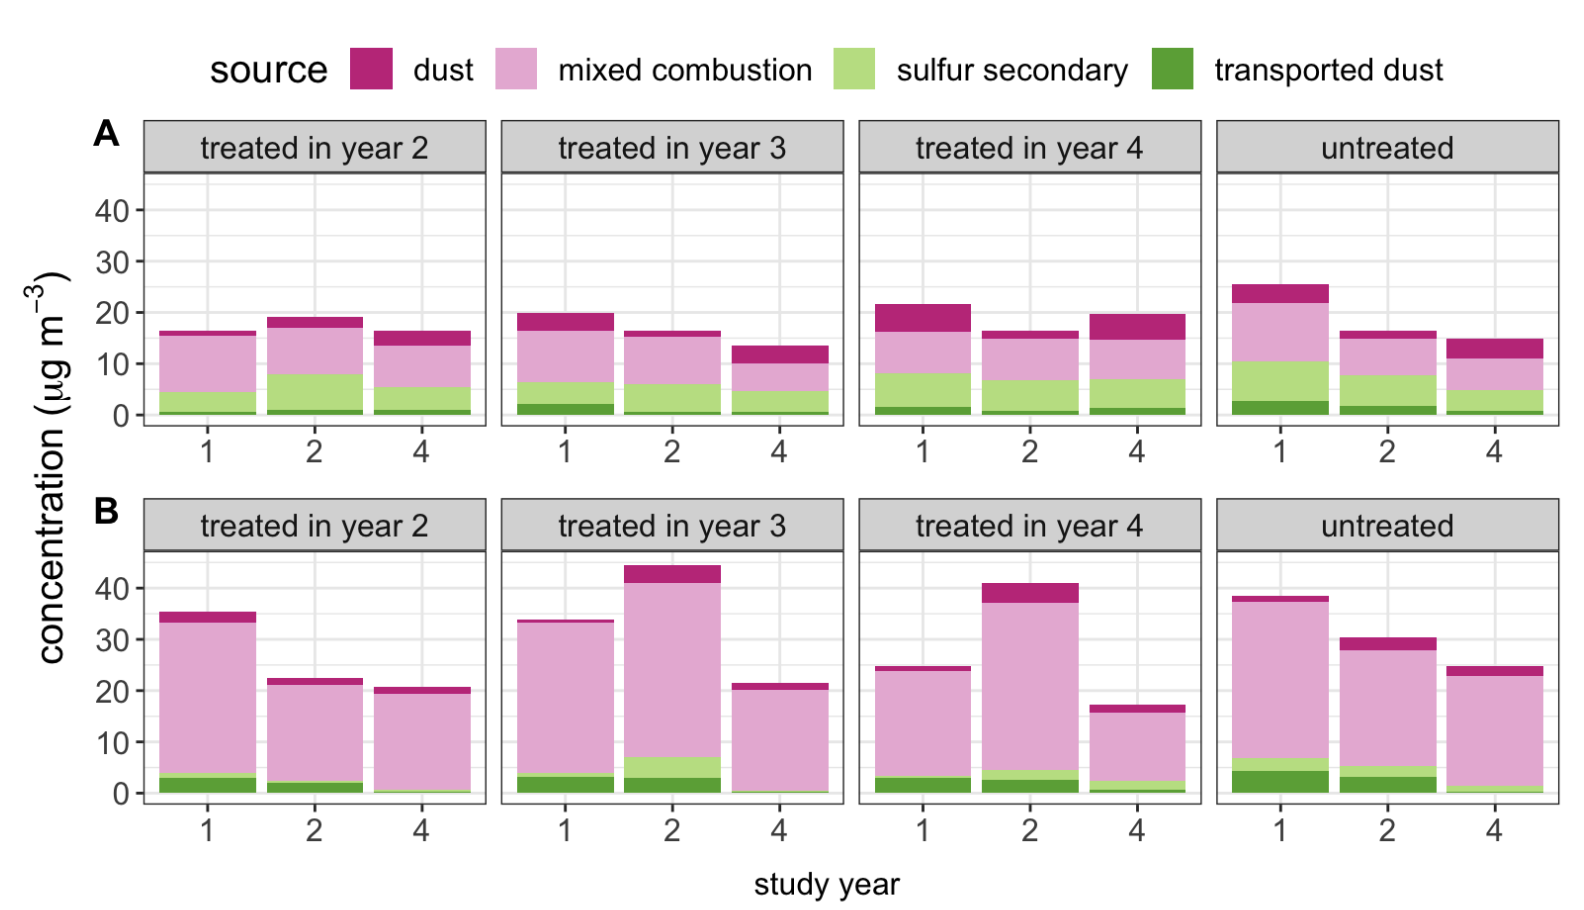
\includegraphics[width=0.8\textwidth,height=\textheight]{images/source-season.png}

}

\caption{\label{fig-source-season}Arithmetic mean dispersion normalized
source contributions found from the 4-factor PMF solution for A outdoor
and B personal PM2.5 exposure samples by year the group received
treatment.}

\end{figure}

\hypertarget{aim-3}{%
\subsection{Aim 3}\label{aim-3}}

\begin{itemize}
\tightlist
\item
  Table of mediated health effects by source contribution (coal and
  biomass)
\end{itemize}

\hypertarget{discussion-and-conclusions}{%
\section{Discussion and Conclusions}\label{discussion-and-conclusions}}

\begin{itemize}
\tightlist
\item
  Generally describing high take-up of the policy
\item
  Reductions in indoor PM\textsubscript{2.5} but not personal or outdoor
\end{itemize}

(Ellison's notes / outline / incomplete discussion -- just trying to get
some structure and key points down). Aim 2 and Aim 3 of this study
focused on investigating the impact of a coal ban on air pollution.
Overall, the results make sense. PM is a mixture of many sources. We
expect that measures of air pollution that are closest to the source
impacted by the policy -- which is stationary and in people's homes --
might be the most likely to reveal the impact of the policy, especially
since the activity most impacted by the policy is also a more
stationary, sustained activity -- i.e., heating. So, it makes sense that
the indoor PM measures show the greatest reduction once the ban was in
place. Further, it makes sense that longer-term measures of indoor PM
show a stronger effect of the ban. Finally, indoor BC did not show as
strong an impact of the ban

(Ellison's notes / outline / incomplete discussion -- just trying to get
some structure and key points down). The most consistent reduction in PM
was observed for indoor, long-duration measurements, suggesting a
successful reduction in indoor air pollution from the coal ban. Discuss
how PM and BC results are coherent with one another (and possibly with
the fuel / energy use trends and results).

(Ellison's notes / outline / incomplete discussion -- just trying to get
some structure and key points down). While there was a lack of
statistically significant reductions in personal PM and outdoor PM,
{[}blah blah blah{]} points to some possible explanations for these
inconclusive findings as well as some interpretations that are
consistent with our overall finding that the CBHP policy was effective.
Personal PM measurements might be more susceptible to short-term
variations in activities or microenvironments. Outdoor PM might be
influenced by regional sources beyond the immediate community where the
ban was implemented.

(Ellison's notes / outline / incomplete discussion -- just trying to get
some structure and key points down). Source Apportionment. Discuss the
finding of reduced mixed combustion source contribution in villages with
more recent treatment. This finding supports the effectiveness of the
ban in targeting a major source of indoor air pollution from coal.
Highlight strengths of dispersion normalization. Briefly mention
limitations of source apportionment analysis (e.g., limited ability to
separate secondary sulfur source and mixed combustion source).

(Ellison's notes / outline / incomplete discussion -- just trying to get
some structure and key points down). Strengths and Limitations of
Measurement Approaches. Acknowledge the use of multiple measurement
approaches (community outdoor, indoor, personal). Explain why we used
these approaches: i.e., to capture a comprehensive picture of air
pollution exposure. Discuss the strengths and limitations of each
approach (e.g., indoor vs personal exposure).

\begin{itemize}
\tightlist
\item
  Reduction in blood pressure and self-reported respiratory symptoms
\end{itemize}

Other relevant results (Tables or figures in SI)

Policy impacts on other relevant outcomes:

\begin{itemize}
\tightlist
\item
  Temperature
\item
  Heating room
\item
  Well-being
\end{itemize}

\hypertarget{implications-of-findings}{%
\section{Implications of Findings}\label{implications-of-findings}}

\hypertarget{data-availability-statement}{%
\section{Data Availability
Statement}\label{data-availability-statement}}

\begin{itemize}
\tightlist
\item
  Description of datasets and code available on our project page at the
  Open Science Foundation
\end{itemize}

\hypertarget{acknowledgements}{%
\section{Acknowledgements}\label{acknowledgements}}

To come\ldots{}

\hypertarget{references}{%
\section{References}\label{references}}

\hypertarget{refs}{}
\begin{CSLReferences}{1}{0}
\leavevmode\vadjust pre{\hypertarget{ref-ahmed2009}{}}%
Ahmed T, Dutkiewicz VA, Shareef A, Tuncel G, Tuncel S, Husain L. 2009.
Measurement of black carbon ({BC}) by an optical method and a
thermal-optical method: {Intercomparison} for four sites. Atmospheric
Environment 43:6305--6311;
doi:\href{https://doi.org/10.1016/j.atmosenv.2009.09.031}{10.1016/j.atmosenv.2009.09.031}.

\leavevmode\vadjust pre{\hypertarget{ref-alexander2018}{}}%
Alexander DA, Northcross A, Karrison T, Morhasson-Bello O, Wilson N,
Atalabi OM, et al. 2018. Pregnancy outcomes and ethanol cook stove
intervention: {A} randomized-controlled trial in {Ibadan}, {Nigeria}.
Environment International 111:152--163;
doi:\href{https://doi.org/10.1016/j.envint.2017.11.021}{10.1016/j.envint.2017.11.021}.

\leavevmode\vadjust pre{\hypertarget{ref-baumgartner2018}{}}%
Baumgartner J, Carter E, Schauer JJ, Ezzati M, Daskalopoulou SS, Valois
M-F, et al. 2018. Household air pollution and measures of blood
pressure, arterial stiffness and central haemodynamics. Heart
104:1515--1521;
doi:\href{https://doi.org/10.1136/heartjnl-2017-312595}{10.1136/heartjnl-2017-312595}.

\leavevmode\vadjust pre{\hypertarget{ref-callaway2020}{}}%
Callaway B. 2020.
\href{https://doi.org/10.1007/978-3-319-57365-6_352-1}{Difference-in-{Differences}
for {Policy Evaluation}}. In: \emph{Handbook of {Labor}, {Human
Resources} and {Population Economics}} (K.F. Zimmermann, ed). Springer
International Publishing:Cham. 1--61.

\leavevmode\vadjust pre{\hypertarget{ref-callaway2021}{}}%
Callaway B, Sant'Anna PHC. 2021. Difference-in-{Differences} with
multiple time periods. Journal of Econometrics 225:200--230;
doi:\href{https://doi.org/10.1016/j.jeconom.2020.12.001}{10.1016/j.jeconom.2020.12.001}.

\leavevmode\vadjust pre{\hypertarget{ref-card1994}{}}%
Card D, Krueger AB. 1994. Minimum {Wages} and {Employment}: {A Case
Study} of the {Fast-Food Industry} in {New Jersey} and {Pennsylvania}.
American Economic Review 84: 772--93.

\leavevmode\vadjust pre{\hypertarget{ref-clark2017}{}}%
Clark S, Carter E, Shan M, Ni K, Niu H, Tseng JTW, et al. 2017. Adoption
and use of a semi-gasifier cooking and water heating stove and fuel
intervention in the {Tibetan Plateau}, {China}. Environmental Research
Letters 12:075004;
doi:\href{https://doi.org/10.1088/1748-9326/aa751e}{10.1088/1748-9326/aa751e}.

\leavevmode\vadjust pre{\hypertarget{ref-costello2015}{}}%
Costello BT, Schultz MG, Black JA, Sharman JE. 2015. Evaluation of a
{Brachial Cuff} and {Suprasystolic Waveform Algorithm Method} to
{Noninvasively Derive Central Blood Pressure}. American Journal of
Hypertension 28:480--486;
doi:\href{https://doi.org/10.1093/ajh/hpu163}{10.1093/ajh/hpu163}.

\leavevmode\vadjust pre{\hypertarget{ref-cdcgr2023}{}}%
Dispersed Coal Management Research Group
北京大学能源研究院气候变化与能源转型项目. 2023. 中国散煤综合治理研究报告
{China Dispersed Coal Governance Report}.

\leavevmode\vadjust pre{\hypertarget{ref-dockery2013}{}}%
Dockery DW, Rich DQ, Goodman PG, Clancy L, Ohman-Strickland P, George P,
et al. 2013. \href{https://www.ncbi.nlm.nih.gov/pubmed/24024358}{Effect
of air pollution control on mortality and hospital admissions in
{Ireland}}. Research Report (Health Effects Institute) 3--109.

\leavevmode\vadjust pre{\hypertarget{ref-dominici2014}{}}%
Dominici F, Greenstone M, Sunstein CR. 2014. Science and regulation.
{Particulate} matter matters. Science (New York, NY) 344:257--9;
doi:\href{https://doi.org/10.1126/science.1247348}{10.1126/science.1247348}.

\leavevmode\vadjust pre{\hypertarget{ref-ezzati2017}{}}%
Ezzati M, Baumgartner JC. 2017. Household energy and health: Where next
for research and practice? Lancet (London, England) 389:130--132;
doi:\href{https://doi.org/10.1016/S0140-6736(16)32506-5}{10.1016/S0140-6736(16)32506-5}.

\leavevmode\vadjust pre{\hypertarget{ref-fda2018}{}}%
Food and Drug Administration. 2018. Bioanalytical {Method Validation
Guidance} for {Industry}.

\leavevmode\vadjust pre{\hypertarget{ref-goin2023}{}}%
Goin DE, Riddell CA. 2023. Comparing {Two-way Fixed Effects} and {New
Estimators} for {Difference-in-Differences}: {A Simulation Study} and
{Empirical Example}. Epidemiology 34:535;
doi:\href{https://doi.org/10.1097/EDE.0000000000001611}{10.1097/EDE.0000000000001611}.

\leavevmode\vadjust pre{\hypertarget{ref-goodman-bacon2021}{}}%
Goodman-Bacon A. 2021. Difference-in-differences with variation in
treatment timing. Journal of Econometrics 225:254--277;
doi:\href{https://doi.org/10.1016/j.jeconom.2021.03.014}{10.1016/j.jeconom.2021.03.014}.

\leavevmode\vadjust pre{\hypertarget{ref-gould2023}{}}%
Gould CF, Bejarano ML, Kioumourtzoglou M-A, Lee AG, Pillarisetti A,
Schlesinger SB, et al. 2023. Widespread {Clean Cooking Fuel Scale-Up}
and under-5 {Lower Respiratory Infection Mortality}: {An Ecological
Analysis} in {Ecuador}, 1990--2019. Environmental Health Perspectives
131:037017;
doi:\href{https://doi.org/10.1289/EHP11016}{10.1289/EHP11016}.

\leavevmode\vadjust pre{\hypertarget{ref-gbdmaps2016}{}}%
Group GMW. 2016. Burden of disease attributable to coal-burning and
other air pollution sources in {China}.

\leavevmode\vadjust pre{\hypertarget{ref-johnson2022}{}}%
Johnson M, Pillarisetti A, Piedrahita R, Balakrishnan K, Peel JL,
Steenland K, et al. 2022. Exposure {Contrasts} of {Pregnant Women}
during the {Household Air Pollution Intervention Network Randomized
Controlled Trial}. Environmental Health Perspectives 130:097005;
doi:\href{https://doi.org/10.1289/EHP10295}{10.1289/EHP10295}.

\leavevmode\vadjust pre{\hypertarget{ref-johnston2013}{}}%
Johnston FH, Hanigan IC, Henderson SB, Morgan GG. 2013. Evaluation of
interventions to reduce air pollution from biomass smoke on mortality in
{Launceston}, {Australia}: Retrospective analysis of daily mortality,
1994-2007. BMJ 346:e8446--e8446;
doi:\href{https://doi.org/10.1136/bmj.e8446}{10.1136/bmj.e8446}.

\leavevmode\vadjust pre{\hypertarget{ref-keele2015}{}}%
Keele L, Tingley D, Yamamoto T. 2015. Identifying mechanisms behind
policy interventions via causal mediation analysis. Journal of Policy
Analysis and Management 34: 937--963.

\leavevmode\vadjust pre{\hypertarget{ref-lai2019}{}}%
Lai. 2019. Relative contributions of household solid fuel use and
outdoor air pollution to chemical components of personal {PM2}.5
exposures. Indoor Air-international Journal of Indoor Air Quality and
Climate.

\leavevmode\vadjust pre{\hypertarget{ref-lewington2012}{}}%
Lewington S, LiMing L, Sherliker P, Yu G, Millwood I, Zheng B, et al.
2012. Seasonal variation in blood pressure and its relationship with
outdoor temperature in 10 diverse regions of {China}: The {China
Kadoorie Biobank}. Journal of hypertension 30: 1383.

\leavevmode\vadjust pre{\hypertarget{ref-lindemann2017}{}}%
Lindemann U, Stotz A, Beyer N, Oksa J, Skelton DA, Becker C, et al.
2017. Effect of indoor temperature on physical performance in older
adults during days with normal temperature and heat waves. International
journal of environmental research and public health 14;
doi:\href{https://doi.org/10.3390/ijerph14020186}{10.3390/ijerph14020186}.

\leavevmode\vadjust pre{\hypertarget{ref-lowe2009}{}}%
Lowe A, Harrison W, El-Aklouk E, Ruygrok P, Al-Jumaily AM. 2009.
Non-invasive model-based estimation of aortic pulse pressure using
suprasystolic brachial pressure waveforms. Journal of Biomechanics
42:2111--2115;
doi:\href{https://doi.org/10.1016/j.jbiomech.2009.05.029}{10.1016/j.jbiomech.2009.05.029}.

\leavevmode\vadjust pre{\hypertarget{ref-mccracken2007}{}}%
McCracken JP, Smith KR, Díaz A, Mittleman MA, Schwartz J. 2007. Chimney
{Stove Intervention} to {Reduce Long-term Wood Smoke Exposure Lowers
Blood Pressure} among {Guatemalan Women}. Environmental Health
Perspectives 115:996--1001;
doi:\href{https://doi.org/10.1289/ehp.9888}{10.1289/ehp.9888}.

\leavevmode\vadjust pre{\hypertarget{ref-mccracken2011}{}}%
McCracken J, Smith KR, Stone P, Díaz A, Arana B, Schwartz J. 2011.
Intervention to {Lower Household Wood Smoke Exposure} in {Guatemala
Reduces ST-Segment Depression} on {Electrocardiograms}. Environmental
Health Perspectives 119:1562--1568;
doi:\href{https://doi.org/10.1289/ehp.1002834}{10.1289/ehp.1002834}.

\leavevmode\vadjust pre{\hypertarget{ref-meng2023}{}}%
Meng W, Zhu L, Liang Z, Xu H, Zhang W, Li J, et al. 2023. Significant
but {Inequitable Cost-Effective Benefits} of a {Clean Heating Campaign}
in {Northern China}. Environmental Science \& Technology 57:8467--8475;
doi:\href{https://doi.org/10.1021/acs.est.2c07492}{10.1021/acs.est.2c07492}.

\leavevmode\vadjust pre{\hypertarget{ref-naimi2014}{}}%
Naimi AI, Kaufman JS, MacLehose RF. 2014. Mediation misgivings:
Ambiguous clinical and public health interpretations of natural direct
and indirect effects. International journal of epidemiology 43:1656--61;
doi:\href{https://doi.org/10.1093/ije/dyu107}{10.1093/ije/dyu107}.

\leavevmode\vadjust pre{\hypertarget{ref-niu2024}{}}%
Niu J, Chen X, Sun S. 2024. China's {Coal Ban} policy: {Clearing} skies,
challenging growth. Journal of Environmental Management 349:119420;
doi:\href{https://doi.org/10.1016/j.jenvman.2023.119420}{10.1016/j.jenvman.2023.119420}.

\leavevmode\vadjust pre{\hypertarget{ref-onakomaiya2019}{}}%
Onakomaiya D, Gyamfi J, Iwelunmor J, Opeyemi J, Oluwasanmi M,
Obiezu-Umeh C, et al. 2019. Implementation of clean cookstove
interventions and its effects on blood pressure in low-income and
middle-income countries: Systematic review. BMJ Open 9:e026517;
doi:\href{https://doi.org/10.1136/bmjopen-2018-026517}{10.1136/bmjopen-2018-026517}.

\leavevmode\vadjust pre{\hypertarget{ref-worldhealthorganization2021}{}}%
Organization WH. 2021. {WHO Global Air Quality Guidelines}: {Particulate
Matter PM2}.5 and {PM10}), {Ozone}, {Nitrogen Dioxide}, {Sulfur Dioxide}
and {Carbon Monoxide}.

\leavevmode\vadjust pre{\hypertarget{ref-quansah2017}{}}%
Quansah R, Semple S, Ochieng CA, Juvekar S, Armah FA, Luginaah I, et al.
2017. Effectiveness of interventions to reduce household air pollution
and/or improve health in homes using solid fuel in low-and-middle income
countries: {A} systematic review and meta-analysis. Environment
International 103:73--90;
doi:\href{https://doi.org/10.1016/j.envint.2017.03.010}{10.1016/j.envint.2017.03.010}.

\leavevmode\vadjust pre{\hypertarget{ref-rosenthal2018}{}}%
Rosenthal J, Quinn A, Grieshop AP, Pillarisetti A, Glass RI. 2018. Clean
cooking and the {SDGs}: {Integrated} analytical approaches to guide
energy interventions for health and environment goals. Energy for
sustainable development : the journal of the International Energy
Initiative 42:152--159;
doi:\href{https://doi.org/10.1016/j.esd.2017.11.003}{10.1016/j.esd.2017.11.003}.

\leavevmode\vadjust pre{\hypertarget{ref-ruiz-mercado2013}{}}%
Ruiz-Mercado I, Canuz E, Walker JL, Smith KR. 2013. Quantitative metrics
of stove adoption using {Stove Use Monitors} ({SUMs}). Biomass and
Bioenergy 57:136--148;
doi:\href{https://doi.org/10.1016/j.biombioe.2013.07.002}{10.1016/j.biombioe.2013.07.002}.

\leavevmode\vadjust pre{\hypertarget{ref-scott2011}{}}%
Scott AJ, Scarrott C. 2011. Impacts of residential heating intervention
measures on air quality and progress towards targets in {Christchurch}
and {Timaru}, {New Zealand}. Atmospheric Environment 45:2972--2980;
doi:\href{https://doi.org/10.1016/j.atmosenv.2010.09.008}{10.1016/j.atmosenv.2010.09.008}.

\leavevmode\vadjust pre{\hypertarget{ref-snider2018}{}}%
Snider G, Carter E, Clark S, Tseng J(TzuW, Yang X, Ezzati M, et al.
2018. Impacts of stove use patterns and outdoor air quality on household
air pollution and cardiovascular mortality in southwestern {China}.
Environment International 117:116--124;
doi:\href{https://doi.org/10.1016/j.envint.2018.04.048}{10.1016/j.envint.2018.04.048}.

\leavevmode\vadjust pre{\hypertarget{ref-song2023}{}}%
Song C, Liu B, Cheng K, Cole MA, Dai Q, Elliott RJR, et al. 2023.
Attribution of {Air Quality Benefits} to {Clean Winter Heating Policies}
in {China}: {Combining Machine Learning} with {Causal Inference}.
Environmental Science \& Technology 57:17707--17717;
doi:\href{https://doi.org/10.1021/acs.est.2c06800}{10.1021/acs.est.2c06800}.

\leavevmode\vadjust pre{\hypertarget{ref-tan2023}{}}%
Tan X, Chen G, Chen K. 2023. Clean heating and air pollution: {Evidence}
from {Northern China}. Energy Reports 9:303--313;
doi:\href{https://doi.org/10.1016/j.egyr.2022.11.166}{10.1016/j.egyr.2022.11.166}.

\leavevmode\vadjust pre{\hypertarget{ref-thompson2019}{}}%
Thompson RJ, Li J, Weyant CL, Edwards R, Lan Q, Rothman N, et al. 2019.
Field {Emission Measurements} of {Solid Fuel Stoves} in {Yunnan}, {China
Demonstrate Dominant Causes} of {Uncertainty} in {Household Emission
Inventories}. Environmental Science \& Technology 53:3323--3330;
doi:\href{https://doi.org/10.1021/acs.est.8b07040}{10.1021/acs.est.8b07040}.

\leavevmode\vadjust pre{\hypertarget{ref-vanderweele2015}{}}%
VanderWeele TJ. 2015. \emph{Explanation in causal inference: Methods for
mediation and interaction}. Oxford University Press:New York.

\leavevmode\vadjust pre{\hypertarget{ref-volckens2017}{}}%
Volckens J, Quinn C, Leith D, Mehaffy J, Henry CS, Miller-Lionberg D.
2017. Development and evaluation of an ultrasonic personal aerosol
sampler. Indoor air 27:409--416;
doi:\href{https://doi.org/10.1111/ina.12318}{10.1111/ina.12318}.

\leavevmode\vadjust pre{\hypertarget{ref-wen2023}{}}%
Wen H, Nie P, Liu M, Peng R, Guo T, Wang C, et al. 2023. Multi-health
effects of clean residential heating: {Evidences} from rural {China}'s
coal-to-gas/electricity project. Energy for Sustainable Development
73:66--75;
doi:\href{https://doi.org/10.1016/j.esd.2023.01.013}{10.1016/j.esd.2023.01.013}.

\leavevmode\vadjust pre{\hypertarget{ref-wooldridge2021}{}}%
Wooldridge JM. 2021. Two-{Way Fixed Effects}, the {Two-Way Mundlak
Regression}, and {Difference-in-Differences Estimators}.;
doi:\href{https://doi.org/10.2139/ssrn.3906345}{10.2139/ssrn.3906345}.

\leavevmode\vadjust pre{\hypertarget{ref-yan2020}{}}%
Yan L, Carter E, Fu Y, Guo D, Huang P, Xie G, et al. 2020. Study
protocol: {The INTERMAP China Prospective} ({ICP}) study. Wellcome Open
Research 4:154;
doi:\href{https://doi.org/10.12688/wellcomeopenres.15470.2}{10.12688/wellcomeopenres.15470.2}.

\leavevmode\vadjust pre{\hypertarget{ref-yap2015}{}}%
Yap P-S, Garcia C. 2015. Effectiveness of {Residential Wood-Burning
Regulation} on {Decreasing Particulate Matter Levels} and
{Hospitalizations} in the {San Joaquin Valley Air Basin}. American
Journal of Public Health 105:772--778;
doi:\href{https://doi.org/10.2105/AJPH.2014.302360}{10.2105/AJPH.2014.302360}.

\leavevmode\vadjust pre{\hypertarget{ref-ye2022}{}}%
Ye W, Steenland K, Quinn A, Liao J, Balakrishnan K, Rosa G, et al. 2022.
Effects of a {Liquefied Petroleum Gas Stove Intervention} on
{Gestational Blood Pressure}: {Intention-to-Treat} and
{Exposure-Response Findings From} the {HAPIN Trial}. Hypertension
79:1887--1898;
doi:\href{https://doi.org/10.1161/HYPERTENSIONAHA.122.19362}{10.1161/HYPERTENSIONAHA.122.19362}.

\leavevmode\vadjust pre{\hypertarget{ref-yu2021}{}}%
Yu C, Kang J, Teng J, Long H, Fu Y. 2021. Does coal-to-gas policy reduce
air pollution? {Evidence} from a quasi-natural experiment in {China}.
Science of The Total Environment 773:144645;
doi:\href{https://doi.org/10.1016/j.scitotenv.2020.144645}{10.1016/j.scitotenv.2020.144645}.

\leavevmode\vadjust pre{\hypertarget{ref-zigler2016}{}}%
Zigler CM, Kim C, Choirat C, Hansen JB, Wang Y, Hund L, et al. 2016.
\emph{Causal inference methods for estimating long-term health effects
of air quality regulations. {Research} report 187.} Health Effects
Institute / Health Effects Institute:Boston, MA.

\end{CSLReferences}

\newpage
\appendix
\renewcommand{\thefigure}{A\arabic{figure}}
\renewcommand{\thetable}{A\arabic{table}}
\setcounter{figure}{0}
\setcounter{table}{0}

\hypertarget{appendices}{%
\section*{Appendices}\label{appendices}}
\addcontentsline{toc}{section}{Appendices}

\begin{figure}[H]

{\centering 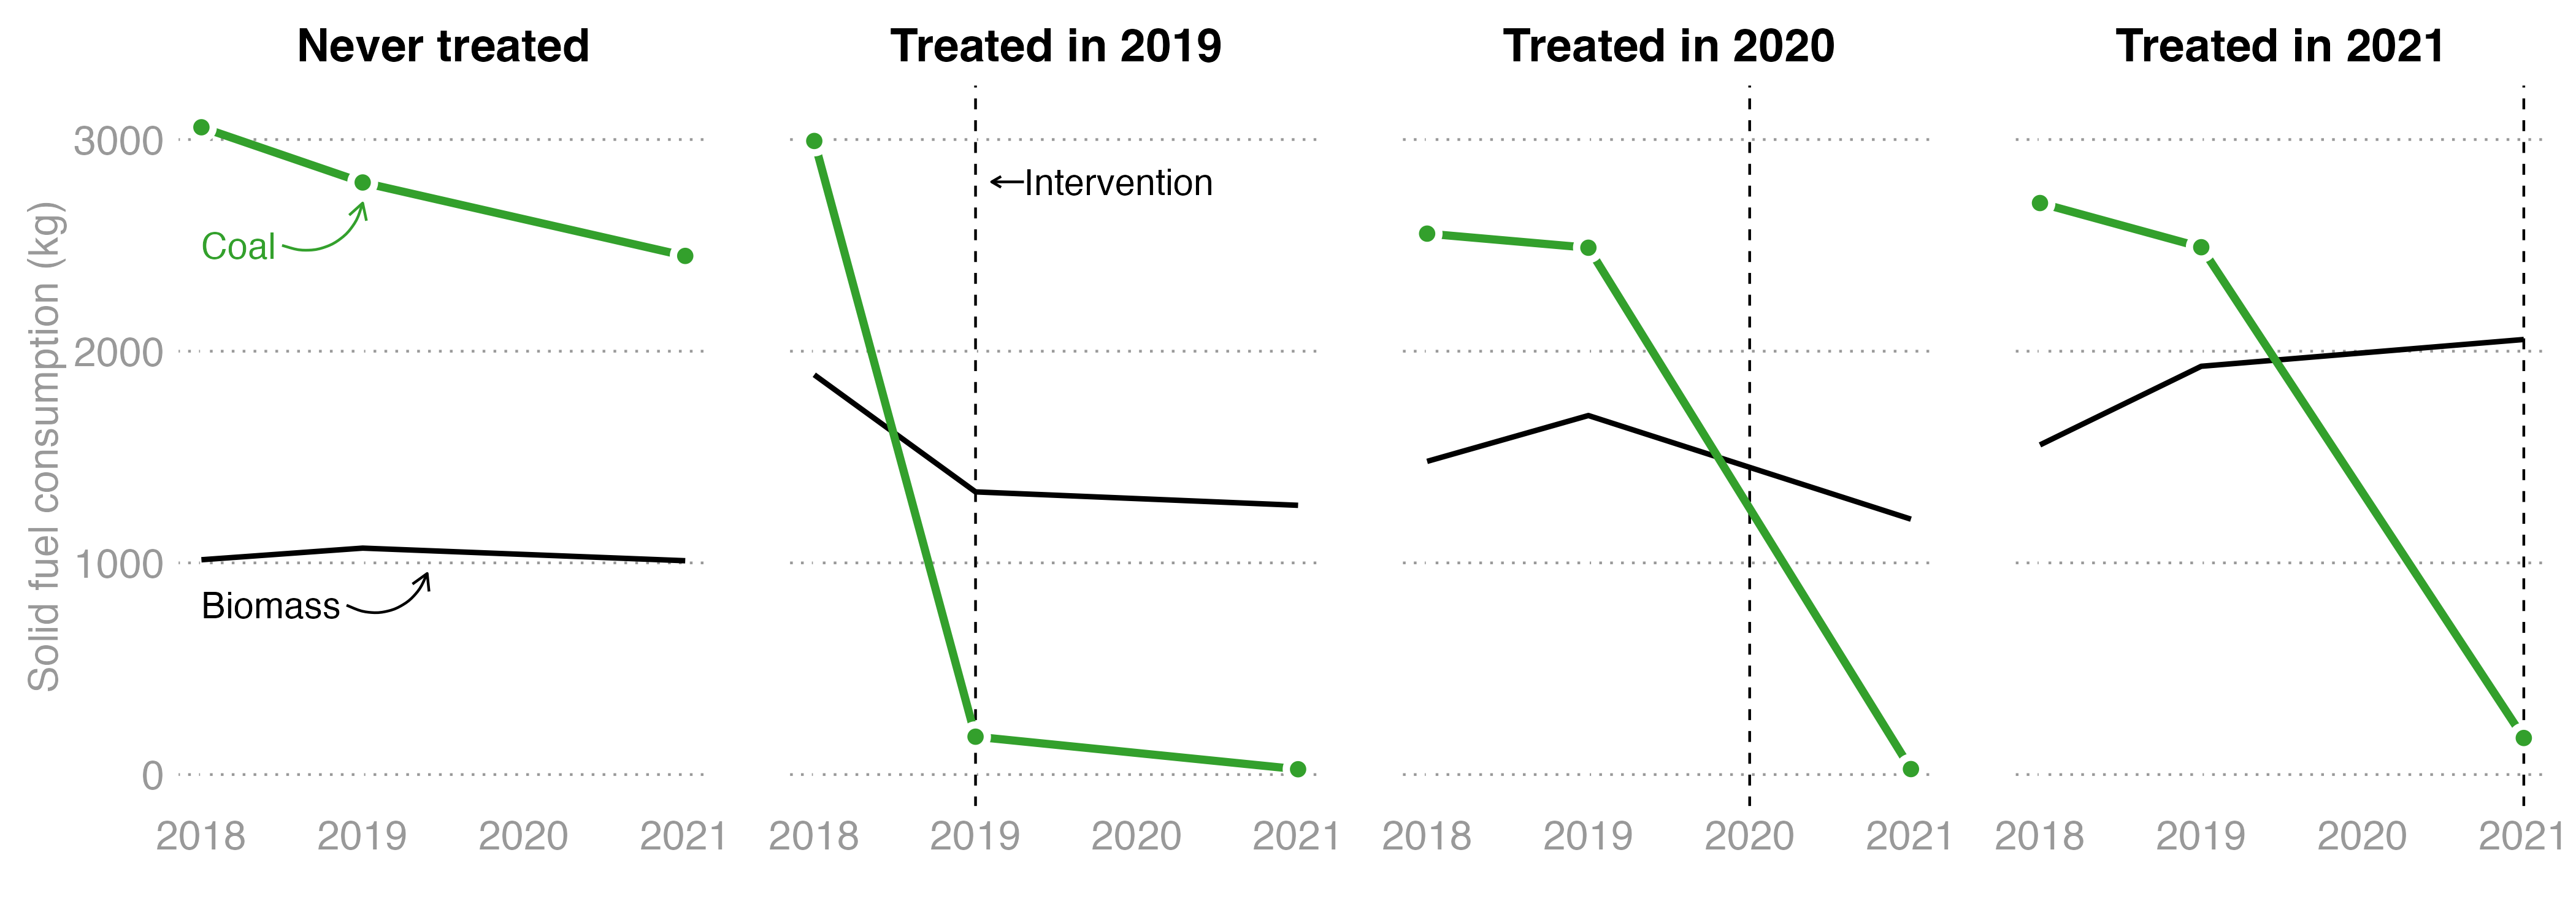
\includegraphics[width=1\textwidth,height=\textheight]{images/coal-plot.png}

}

\caption{\label{fig-afig-coal}Trends in self-reported coal and biomass,
by treatment season}

\end{figure}

Sensitivity analyses: {[}{[}{[}Jill to edit this table include all
sensitivity analysis for total effects models{]}{]}{]}

\begin{verbatim}
Number of participants (observations)
Mean change or percent change in FeNO (ppb)
Limited to participants with two or more measurements
142 (569)
-0.2 [-3.0, 2.5]
Limited to participants with three measurements
95 (285)
0.4 [-2.8, 3.6]
Analysis with log-transformed outcome [ln(FeNO)]
511 (843)
-3.8% [-16.9, 11.4]
\end{verbatim}

\hypertarget{about-the-authors}{%
\section*{About the authors}\label{about-the-authors}}
\addcontentsline{toc}{section}{About the authors}

\hypertarget{other-publications}{%
\section*{Other publications}\label{other-publications}}
\addcontentsline{toc}{section}{Other publications}



\end{document}
